\documentclass[10pt,openany,oneside]{book}
\usepackage[left=1in,right=1in,top=1in,bottom=1in,headheight=14pt,headsep=14pt]{geometry}

\usepackage[draft]{checked_c}

\usepackage{bytefield}
\usepackage{xspace}

\title{Putting the Checks into Checked C \\%
Checked C Technical Report Number 2}

\author{Archibald Samuel Elliott}

\date{31 October 2017}

\hypersetup{%
pdftitle={Putting the Checks into Checked C},
pdfauthor={Archibald Samuel Elliott},
pdfsubject={Checked C Technical Report Number 2}
}

\allowdisplaybreaks

% Auto Generated by bm_res.r
% Do Not Modify
\newcommand{\ResultLinesModifiedMean}{17.5\%\xspace}
\newcommand{\ResultLinesModifiedMax}{35.3\%\xspace}
\newcommand{\ResultLinesModifiedMin}{9.8\%\xspace}

\newcommand{\ResultEasyModificationsMean}{80.1\%\xspace}
\newcommand{\ResultEasyModificationsMax}{98.5\%\xspace}
\newcommand{\ResultEasyModificationsMin}{51.5\%\xspace}

\newcommand{\ResultLinesUncheckedMean}{9.3\%\xspace}
\newcommand{\ResultLinesUncheckedMax}{20.4\%\xspace}
\newcommand{\ResultLinesUncheckedMin}{3.9\%\xspace}

\newcommand{\ResultRunTimeMean}{8.6\%\xspace}
\newcommand{\ResultRunTimeMax}{49.3\%\xspace}
\newcommand{\ResultRunTimeMin}{0.0\%\xspace}

\newcommand{\ResultCompileTimeMean}{24.3\%\xspace}
\newcommand{\ResultCompileTimeMax}{83.1\%\xspace}
\newcommand{\ResultCompileTimeMin}{4.9\%\xspace}

\newcommand{\ResultExecutableSizeMean}{7.4\%\xspace}
\newcommand{\ResultExecutableSizeMax}{26.7\%\xspace}
\newcommand{\ResultExecutableSizeMin}{-5.0\%\xspace}


\begin{document}

\frontmatter
\begin{titlepage}
\begin{center}
\vspace*{2in}
{\huge Putting the Checks into Checked C \\}
\vspace{0.5in}
{Checked C Technical Report Number 2\medskip\\}
{\makeatletter\@date\makeatother\\}
\vspace{0.25in}
{\large Archibald Samuel Elliott\medskip\\}
{Paul G. Allen School,\\
University of Washington\\}
\vspace{1in}
{\it Summary \par}
\begin{minipage}{5in}
Checked C is an extension to C that aims to provide a route for
programmers to upgrade their existing C programs to a safer language
without losing the low-level control they enjoy. Checked C currently
only addresses unsafe code with spatial memory violations such as
buffer overruns and out-of-bounds memory accesses. \\[1em]

Checked C addresses these memory safety problems by adding new pointer
and array types to C, and a method for annotating pointers with
expressions denoting the bounds of the objects they reference in
memory. To ensure memory safety, the Checked C compiler uses a mixture
of static and dynamic checks over these additions to the C language. \\[1em]

This Technical Report concerns these Dynamic Checks, and the
algorithms and infrastructure required to support them, including: the
soundness property Checked C is aiming to preserve, propagation rules
for bounds information, and the code generation algorithm for the
checks themselves. This report includes an evaluation of these dynamic
bounds checks, their overhead, and their interaction with a
state-of-the-art optimizer. 

%%% Local Variables:
%%% mode: latex
%%% TeX-master: "tr02"
%%% End:

\end{minipage}
\end{center}
\end{titlepage}

\tableofcontents

\mainmatter
% !Tex root = checkedc.tex

\chapter{Introduction}
\label{chapter:introduction}

The C programming language \cite{Ritchie1988, ISO2011} allows programmers to use
pointers directly. A pointer is an address of a location in memory. Programs may do
arithmetic on pointers, dereference them to read memory, or assign
through them to modify memory. The ability to use pointers directly
makes C well-suited for low-level system programming that is ``close to
the hardware'' and allows programmers to write efficient programs. C
also unifies pointer types and array types. They can usually be used
interchangeably and array subscripting is a synonym for equivalent
pointer operations.

Pointers and the unification of arrays and pointers are one of the
strengths of the C programming language, allowing programmers to write
concise, efficient programs. At the same time, they are a source of
reliability and security problems in modern software. This is
because pointers and array indices are not bounds checked in C and
related languages such as C++. Bounds checking checks that a pointer or
array index is in bounds before it is used to read or write memory. A
pointer to an array object is in bounds if it points to an element of
the array object. An array index is in bounds if the index is greater
than or equal to zero and less than the size of the array.

Between 2010 and 2015, buffer overflows accounted for between 10-16\% of
publicly reported security vulnerabilities in the U.S. National
Vulnerability Database each year \cite{NIST2015}. The vulnerabilities have affected
software implemented in C and C++ that is widely used, including the
Windows and Linux operating systems, the Internet Explorer, Chrome, and
Safari web browsers, the Apache web server, the OpenSSL security
library, scripting language implementations for Bash, Ruby, and PHP, and
media playback software such as QuickTime.

Because pointers and array indices are not bounds checked in C, a
programming error involving them may corrupt memory locations used by
the program. The memory locations may hold data that is important to the
computations being done by the program or data that is essential to the
control-flow of the program, such as return address locations and
function pointers. Memory corruption can lead to a program producing
incorrect results or, in the hands of a malicious adversary, the
complete malfunctioning of the program and the takeover of a running
process by the adversary.

This technical report describes Checked C, an extension to C that provides
bounds checking for pointers and arrays. There are two obstacles to
adding bounds checking to C. First, it is not clear where to put the
bounds information at runtime. Second, it is not clear how to make the
bounds checking efficient for programs where performance matters. The
solution of changing the representation of all C pointer types and
arrays to carry bounds information is not sufficient in practice. C may
be used at the base of systems where hardware or standards dictate data
layout and data layout cannot be changed. C programs must also
interoperate with existing operating systems and software that require
specific data layouts.

\section{Overview}
Checked C addresses the bounds checking problem for C by:

\begin{itemize}
\item
  Introducing different pointer types to capture the different ways in
  which pointers are used. The unchecked C pointer type \code{*} is kept
  and three new {\it checked} pointer types are added: one for pointers
  that are never used in pointer arithmetic and do not need bounds
  checking (\ptr),  one for \emph{array pointer types} that are involved
  in pointer arithmetic and need bounds checking (\arrayptr), and an
  extension to \arrayptr\ for null-terminated arrays (\ntarrayptr).
\item
  For array pointer types (\arrayptr), in keeping with the low-level
  nature of C,  bounds checking is placed under programmer control.
  This differs from languages like
  Java, where bounds checking is completely automatic. A programmer
  declares \emph{bounds}, where the bounds for an \arrayptr\
  variable are given by non-modifying C expressions. These are a subset
  of C expressions that do not modify variables or memory. They include
  local variables, parameters, constant expressions, casts, and
  operators such as addition, subtraction, and address-of (\code{&})
  operators. Static checking ensures that programs declare and maintain
  bounds information properly. The bounds are used at runtime for
  bounds checking.  A runtime bounds check may be optimized away by a
  compiler if the compiler can prove the check always succeeds.
\item
  Introducing different array types to distinguish between arrays whose
  accesses are bounds-checked and existing C arrays whose accesses are
  not bounds-checked. A programmer places the modifier \keyword{checked}
  before the declaration of the bound(s) of the array: \code{int x
  checked[5][5]} declares a 2-dimensional array for which all
  accesses will be bounds-checked.  Arrays with null terminators
  as their last element can be declared using \keyword{nt\_checked}
  instead of \keyword{checked}.
\item
  For structure types with \arrayptr -typed members, a
  programmer declares \emph{member bounds} for those members. A member
  bounds declares the bounds for a member in terms of members of the
  structure type. Member bounds can be suspended temporarily for
  specific variables and objects. Static checking ensures that updates
  to members maintain the member bounds.
\item
  Introducing bounds-safe interfaces to address the problem of
  interoperation between checked code and unchecked code. A bounds-safe
  interface describes the checked interface to unchecked code by declaring
  bounds for unchecked pointers in function signatures and data structures.
  It describes a boundary that is ``checked'' or ``unchecked''
  depending on what kind of code is using it. The
  interface is trusted in checked code (code that uses only checked pointer types).
  Proper usage is enforced via checking at compile time and runtime. For
  code that uses only unchecked pointer types, the interface is descriptive and
  not enforced by
  language checking. This provides a way to upgrade existing code to
  provide a checked interface without breaking existing users of the code.
\item
  Introducing checked program scopes, where bounds checking is the
  default behavior. In a checked program scope, definitions of variables
  and functions can use checked pointer types and cannot use unchecked pointer
  types. Declarations involving unchecked pointer types must provide
  bounds-safe interfaces. Checked program scopes avoid problems with
  subtle misuse of bounds-safe interfaces.
\item
  Reasoning about the correctness of programs with declared bounds
  sometimes requires reasoning about simple aspects of program behavior.
  To support this, lightweight invariants are added to Checked C. A lightweight
  invariant declares a relation between a variable and a simple
  expression using a relational operator. An example would be the
  statement \code{x < y + 5}. Lightweight invariants can be
  declared at variable declarations, at assignment statements, for
  parameters, and for return values. Checked C is extended with rules for
  checking these lightweight invariants. Just as type checking rules are
  defined by the programming language, so are rules for checking
  lightweight invariants. The checking of the correctness of
  programmer-declared bounds is integrated with the checking of
  invariants.
\item
  For the cases where static checking reaches its limits, a programmer
  can introduce dynamic checks that are runtime errors if they fail.
  Dynamic checks use the syntax \keyword{dynamic\_check} \var{e}, where \var{e} is an
  integer-valued expression. A check is similar to an assert, except
  that it is never removed from the program (unless a compiler proves
  it is redundant). It cannot be removed because the integrity of the
  program depends upon it.
\end{itemize}

For an existing C program to be correct, there has to be an
understanding on the part of the programmer as to why pointers and array
indices stay in range. The goals of the design are to let the programmer
write this knowledge down, to formalize existing practices, such as
array pointer parameters being paired with length parameters, and to
check this information.

To simplify bounds and reasoning about bounds for
\arrayptr\ types, pointer arithmetic overflow for \arrayptr\
types is considered a runtime error. Pointer arithmetic involving a null
pointer for \arrayptr\ types is also a runtime error.

Efficiency is addressed by extending the static checking so that it can
guarantee that specific bounds checks will always succeed at runtime for
\arrayptr\ . The static checking
supports the scenario of simple control-flow enclosing the bounds check
guaranteeing that the bounds check will succeed. For example, a for-loop
may iterate only over values within the declared bounds of an
\arrayptr\ variable.

A problem with incorporating static checking into a programming language
is that static checking needs to be something that compilers can do
quickly and deterministically. Static checking can become very expensive
to do, depending on the language of invariants and the inference that
compilers are expected to do. For example, Presburger arithmetic is
integer arithmetic restricted only to addition and less than or equal
operations. It is NP-complete to determine whether a formula in the
first-order logic for quantifier-free Presburger arithmetic is
always true. Even statically checking properties of
simple fragments of real programs can be computationally intractable.

This problem is addressed in two ways. First, the language rules that are
used to check the validity of bounds are limited intentionally.  The rules can
check the validity of bounds that are needed in practice.  However, there are
bounds that are true that cannot be proved using the rules.  In the terminology
of program logics, the rules are incomplete.  As an example, the
rules about distributivity limit the size of
expressions that they produce.   In practice, this means that
simple disjunctive bounds can be checked, but complex disjunctive bounds cannot be checked.

Second, the inference that compilers do for checking program invariants is
limited.  Compilers act as \emph{checkers} for invariants. They check that
declared invariants follow from other declared invariants, the
program control-flow, intervening assignments, and simple axioms about
invariants, such as transitivity of relational operators. Compilers
do not try to devise invariants or prove the correctness of
invariants; they apply simple local reasoning to check them. The
programmer has to call out the relevant facts. If a programmer declares
an invariant \code{x == y} but neglects to declare the invariant
\code{y == z}, a checker may not be able to reason several
statements later that \code{x == z}, even though it may be true at
that point in the program. This is taking advantage of the fact that
checking a proof is usually much easier than creating the proof.

Establishing the bounds-safety of pointer operations is just the first step in
establishing type safety for C programs. There are other ways which C
programs may fail. C programs may incorrectly deallocate memory that is
still in use, do incorrect type-unsafe pointer casts, or have concurrency
races that tear data structures. Addressing these problems is beyond the
scope of this technical report. For now, it is assumed that programs are
correct in these other aspects.

This design is being done in an iterative fashion.  To validate the
design, we mocked up modifying a subset of the OpenSSL
code base \cite{OpenSSL2015} to be bounds-safe.
We created C++ templates for the new pointer types and modified OpenSSL to
compile as valid C++ code.
We hand-edited about 11,000 lines of the code to use checked pointer
types with full bounds annotations.  We used macros to encapsulate
the bounds annotations so that they could be elided from the code
and OpenSSL compiled and tested using the new types.  We also modified the
generic stack type in OpenSSL to use the \code{ptr} type, which required
cross-cutting changes across the code base (in all, about 160 files were changed)
as well dealing with complicated macros.

We learned the following from this
experience.   First, it was important to have a compact, succinct syntax
for declaring bounds.
Second, in most cases, declaring bounds at declarations was sufficient for
tracking the bounds of variables.  Large blocks of code
remained unchanged, which matches the observations of the
Cyclone project \cite{Jim2002}, an earlier research
effort to create a type-safe version of C.
Third, the expressions allowed in declaring
bounds needed to be rich.  Fourth, pointer casts were used
fairly extensively, but often times it was obvious that the casts were
correct with respect to bounds.  The existing bounds could be modified
easily to be appropriate for the new referent type of the pointer.
Fifth, it was clear that there needed
to be a graceful way of interoperating with existing libraries that could
not be changed.   Finally, signed integer overflow was a pervasive
possibility, which raised questions about the meaning of bounds
declarations that used signed integers.

We revised the design to
address these issues.  In particular, we paid close attention to
tracking bounds through pointer casts.  We also made sure that the
constraints on signed integer expressions used in bounds expressions
were understood and could be written down in the language of
simple invariants.

\section{Principles for extensions}
\label{chapter:principles}

Here are the principles that are followed to extend C to support bounds checking:

\begin{enumerate}
\item
  Preserve the efficiency and control of C. C is designed to be
  low-level and work with the same types that computer processors work
  with. This allows programmers to
  control what programs do precisely at the
  machine level. This efficiency and control are reasons why C is valued as a
  system programming language. Extensions will be ``pay-as-you-go'' and
  continue to provide precise control to programmers at the machine
  level. Hidden costs will be avoided.
\item
  Be Minimal. This means adding the minimal set of extensions needed to
  accomplish the goals. It is easier to learn extensions if there are as
  few of them as possible. It also stays true to the design goals
  of C.
\item
  Aim for clarity and succinctness. Clarity means that code is easy to
  understand and extensions are straightforward to understand.
  Succinctness means the programmers have less to read or type.
  Programmers value clarity and succinctness because it makes them more
  productive.  Sometimes clarity and succinctness are in
  tension and sometimes they are not. When they are in conflict, clarity
  will be prioritized above succinctness, primarily because source code
  is usually read many more times than it is written.
\item
  Enable incremental use. Real systems are large and complicated, with
  hundreds of thousands and millions of lines of code. The teams that
  work on those systems will adopt checked pointer operations over time,
  not all at once, so incremental use of checked pointer operations will be
  supported. Teams will prefer incremental conversion paths because of
  practical matters such as reducing risk, fixing existing bugs
  identified by introducing bounds checking, maintaining system
  stability, and understanding performance effects. Even though
  incremental use will be supported, it is not the end goal. We believe
  that benefits of using checked pointer operations will be modest until
  almost an entire system is converted. At that point, we expect a
  qualitative increase in system reliability and programmer
  productivity.
\end{enumerate}

Two specific design principles are adopted based on these principles:

\begin{enumerate}
\item
  Do not change the meaning of existing C code. Methods that do not use
  extensions will continue to compile, link, and run ``as is''. If the
  meaning of existing C code is changed, it will violate the principles
  of clarity and enabling incremental adoption.
\item
  Adopt existing notations from C++ when they meet our needs, instead of
  inventing new notations. Many systems are hybrid C/C++ systems, so
  this approach fits with the principle of clarity. It also enables
  incremental adoption. One of the design goals of C++ has been that C
  is a subset of C++.  It is a design goal to allow Checked C extensions
  to be amenable to being added to C++ too, so that Checked C is a subset
  of a Checked C++.
\end{enumerate}

\section{Notation}
This specification includes many code examples.   Code will be shown in a teletype font (like \texttt{\small this}).
Operators and symbolic characters will be shown in black (like \lstinline|->|).    Keywords will be shown in blue and program
variables will be shown in light blue (like \lstinline|for (int i = 0; i<10; i++)|).   At times, we will
define properties or make mathematical statements that range over sets of values or program
elements, such as mathematical integers, variables, or expressions.   We will use meta-variables in {\it italics} that
range over these values or program elements.  We might say something like
``for all expressions \var{e\textsubscript{1}} and \var{e\textsubscript{2}}.''   These meta-variables
 differ from program variables, which are elements of specific C programs.

\section{Organization of this document}

Chapter~\ref{chapter:core-extensions} describes
the new pointer types and the new array types, including syntax,
semantics, and error conditions. It also covers other extensions to C
semantics. One extension is the introduction of checked program scopes to
prevent inadvertent use of unchecked types. Another extension is a
refinement of C's notion of undefined behavior. We wish to maintain
bounds safety even in the face of integer overflow, which is a
widespread possibility in C programs. This requires a more nuanced
requirement on the result of overflow than ``the result is undefined.''

Chapter~\ref{chapter:tracking-bounds} describes how programmers declare the bounds for
\arrayptr\ variables and structure members. It also describes the meaning of bounds declarations.
Bounds can be declared at variable declarations. They can also be
declared for local variables at expression statements. If the only
bounds declaration for a variable is at the declaration of the variable,
the bounds declaration is an invariant bounds declaration that is true 
for the lifetime of the variable. If there are bounds declarations for the
variable at assignments or other declarations, all bounds declarations for the variable are
dataflow-sensitive. Dataflow-sensitive bounds declarations extend via
dataflow to uses of the variable.

Invariant bounds declarations must usually be valid after every
statement and declaration in the scope of a variable. Sometime multiple
statements are needed to update the variables in a bounds
declaration.
To support this, expression statements and
declarations can be be replaced in \emph{bundled} block, in which
case bounds declarationsmust be valid only at the end of the block.
In the bundled block, the variables may be inconsistent with respect to
bounds declarations that use them. 

Member bounds declarations are type-level invariants about members
of structure types. We assume that that concurrency control is
been done correctly for those data structure.  Race conditoin in
updates could make the type-level invariants invalid.

When pointers to structure are used to modify members, Checked C requires
that modifications to members preserve type-level bounds invariants.
This follows the lead of the Deputy system \cite{Condit2007}.

Chapter~\ref{chapter:interoperation} covers interoperation between
checked and unchecked code. It covers conversions between checked and
unchecked pointers, as well as conversions between the new kinds of checked pointers.
It pins down the notion of checked code  and unchecked code. Finally, it covers
bounds-safe interfaces in depth.

Chapter~\ref{chapter:checking-bounds} describes rules that the compiler uses to check the validity
of bounds declarations. It covers inferring bounds for expressions.
Because expression may have assignments embedded within them, it also
covers inferring effects of an expression on the bounds of variables.
This inferred information is then used to validate that declarations and
statements correctly declare bounds and maintain the bounds information.

Chapter~\ref{chapter:simple-invariants}
extends the checking of bounds to incorporate simple
reasoning about bounds and program behavior. It includes a set of rules
for deducing facts that are true about a program at a specific point in
the program (for example, given an assignment \code{x = y;} the fact
that x == y is true after the assignment). Facts can also be deduced
from program control-flow. There are additional rules for reasoning
about whether one fact is true given a set of other facts (for example,
given x == y and the statement \code{z = y;} z == x is true after that
statement). These rules and facts can be used to deduce the correctness
of bounds declarations that differ from those inferred directly by the
checking described in Chapters~\ref{chapter:checking-bounds}. For example,
a programmer may wish to narrow the memory that is accessible via an
\arrayptr\ variable by declaring bounds that are a subrange of
the bounds inferred by the checking. A programmer may wish to update the
bounds for an \arrayptr\ variable after an assignment \code{x = y}, substituting
\code{x} for \code{y}.

The same static checking that is used for bounds can be used to reason
about the ranges of variables at specific points in a program. From
there, it is a short step to deducing at compile-time that bounds are
always satisfied at a particular memory access in a program. For
example, a fact can be that the range of an integer variable \code{i}
is always between 0 and 10. This can be used to deduce that an array
access in a crucial inner loop is always in bounds.

Chapter\ref{chapter:roadmap} describes future planned features for Checked C.
These feature are currently not implemented in the Checked C compiler.

\omitted{
Chapter~\ref{chapter:eval} evaluates the design by describing our experience modifying
an existing C open-source code base by hand to use the Checked C
extensions. We chose to modify OpenSSL, an important widely-used
open-source code base. The static and dynamic checking is not
implemented in a compiler yet, so we cannot be sure of the correctness
of the modifications or understand the practical benefits of checking.
Still, this gives some idea about the usefulness and applicability of
the design.

Chapter~\ref{chapter:open-issues} summarizes the open problems uncovered by
Chapter~\ref{chapter:eval} or
unaddressed by the design. It also describes next steps for implementing
this in a C compiler.
}

Appendix~\ref{chapter:related-work} describes related work that addresses
the lack of bounds checking in C.  Because of the serious practical consequences
for computer security and software reliability, there has been extensive work
in the area.  We are heavily influenced by the Deputy system \cite{Feng2006,Condit2007}.

Appendix~\ref{chapter:design-alternatives} discusses design alternatives
that were considered and not chosen.  It explains why those alternatives were
not chosen.

\section{Acknowledgements}

This design has benefited from many discussions with Weidong Cui, Gabriel Dos Reis,
Sam Elliott, Chris Hawblitzel, Galen Hunt, Shuvendu Lahiri, and Reuben Olinsky.  The design has
benefited also from feedback from Michael Hicks, Wonsub Kim, Greg
Morrisett, Jonghyun Park, and Andrew Ruef. We thank them for their contributions to
the design.



\chapter{Overview of Checked C}
\label{sec:checkedc}

Checked C is an extension to C that adds static and dynamic checking
to prevent and detect common programming errors such as buffer
overruns, out-of-bounds memory accesses, and incorrect type casts.
Given that it is an extension to C, it aims to preserve backwards
compatibility with C11~\cite{ISO2011}.

This report is concerned with how Checked C prevents buffer overruns
and out-of-bounds memory accesses. In order to reason about these
behaviours, Checked C adds new data types, a method to annotate
variable declarations with a static description of their runtime
bounds, checked regions, new casts, and a method for interoperation
with and describing existing C code.

It is this static bounds description, which we call a ``bounds
expression'', that is used both during static analysis and during code
generation for the dynamic checks, and that we consider to be the main
idea underlying Checked C's approach.

\section{New Data Types}

Checked C adds new types to C:

\begin{itemize}
\item \PtrT, the checked pointer to singleton type,
\item \ArrayptrT, the checked pointer to array type,
\item \CheckedarrT{\mv{N}}, the checked array type,
\end{itemize}

Both the checked pointer to singleton and the checked pointer to
array types are intended to replace most uses of C's \uncheckedptrT,
which we call the unchecked pointer type. The checked array type is
intended to replace most uses of C's \uncheckedarrT{\mv{N}}, which we
call the unchecked array type.

The checked pointer to singleton type, \PtrT, is intended to replace
uses unchecked pointer types that are a
pointer to a single value of type \mv{T}. For this reason, it is
illegal to perform any pointer arithmetic on a value of type \PtrT,
including array indexing. Checked pointers to singletons require no
bounds checks, but may be null.

The checked pointer to array type, \ArrayptrT, is intended to replace
uses of the equivalent unchecked pointer type, where it is used as a
pointer to an array of values of type \mv{T}. These pointers may be
null, may not overflow on pointer arithmetic, and require bounds
checks when they are used to access memory.

The checked array type, \CheckedarrT{\mv{N}}, is intended to replace
uses of the equivalent unchecked array type, \uncheckedarrT{\mv{N}}.
In the same way that there is a duality between C's unchecked arrays
and unchecked pointers, there is the same duality between Checked C's
checked pointers to arrays and checked arrays.

We place two restrictions on the checked array type,
\CheckedarrT{\mv{N}}. First, they may not be variable length, so
\mv{N} must be a compile-time constant. Second, if an outer
dimension of a multidimensional array is checked, all dimensions
inside that dimension are also checked.

\section{Bounds Expressions}

In order to denote the bounds on a declaration or parameter, a bounds
expression is associated with a checked array or checked array
pointer, such as the bounds annotation at~\lstref{main:count}
in~\autoref{lst:checked-main}.

\begin{code}[label=lst:checked-main,%
caption={Declaration of \lstinline|main| in a Checked C program}]
int main(int argc, array_ptr<char*> argv : count(argc) ~\lstlabel{main:count}~);
\end{code}

\autoref{lst:checked-main}, though very short, shows several features
of Checked C. The first is that Checked C's new types work exactly how
C's regular types already do. The next feature is that we can annotate
function parameters of pointer type with a bounds expression that
provides a static description of that parameter's runtime bounds. The
bounds expression at~\lstref{main:count} is only for the outer
\ArrayptrT, it does not apply to the inner unchecked pointer.

The last feature is the bounds expression itself. There are three
forms of bounds expressions in Checked C. The first, called a ``count
expression'' is shown above --- here it denotes that the array has
\lstinline|argc| elements. There is a more complicated bounds
expression called a ``range expression'', which is written
\bounds{\mv{lower}}{\mv{upper}} and denotes that the associated
pointer is within the range $[\mv{lower}, \mv{upper})$. The last form
of a bounds expression is written \boundsbytecount{\mv{n}} and means
the array pointer points to the start of an array \mv{n} bytes long,
regardless of the element size.

In~\autoref{lst:checked-main}, we could not declare \lstinline|argv|
to have type \Checkedarr{\expr{\kw{char}*}}{\mv{argc}}, as
\lstinline|argv| checked arrays may not be variable-length. It is also
not \uncheckedarr{\Checkedarr{\kw{char}}{\mv{argc}}}{}, both as this
declares the outer array as variable-length, and as this requires the
inner array to be checked, but we have no information as to its length
as it is a null-terminated string.\endnote{In fact, in C, no function
parameter has array type, as you cannot pass an array (checked or not)
to a function. Arrays are passed by passing a pointer to their first
element, so C functions that are declared to have array-typed
parameters actually have the equivalent pointer-typed parameter.
Checked C does the same with checked arrays and checked pointers to
arrays respectively.}

It is an error for a Checked C program to access memory via a null
checked pointer, so these bounds only apply if the pointer is
non-null.

\section{Explicit Cast Operators}
\label{sec:dynamiccastops}

The logic of Checked C's bounds checks is reliant on C's expression
semantics. Notably, this logic is undecidable, especially when it
comes to deciding if one bounds expression implies another. We would
prefer if compiling did not take infinitely long, so Checked C includes
two operators that a programmer may use when the compiler requires,
but cannot prove, that one bounds expression is a sub-range of
another. These assert to the compiler that an expression has
particular bounds, and are our ``bounds cast'' operators (in the same
way a type cast operator asserts to the compiler that an expression
has a particular type). \autoref{sec:static-checks} describes exactly
when the compiler needs to prove these implications.

The dynamic bounds cast operator,
\dynamiccast{\mv{T}}{\mv{e}}{\mv{lb}}{\mv{ub}}, performs a cast to
type \mv{T} and a dynamic check to make sure that either \mv{e} is
\NULL, or that the required bounds, $\left[\mv{lb}, \mv{ub}\right)$,
are a sub-range of the bounds of \mv{e}. This check is explicit so that
the programmer can see where there is an overhead in their program.
Effectively this asserts a fact that will later be verified at run time.

The assume bounds cast operator,
\assumecast{\mv{T}}{\mv{e}}{\mv{lb}}{\mv{ub}}, has the equivalent
compile-time behaviour of the dynamic bounds cast operator, but
performs no run-time check. This is used to assert to the compiler
that \mv{e} really has bounds $[\mv{lb}, \mv{ub})$, without incurring
run-time overhead. This asserts a fact that will never be verified,
and is therefore a potential source of unsoundness.

\section{Checked Regions}
\label{sec:checked-regions}

Checked C programs contain regions of unchecked and checked code. By
default, all code is within an unchecked region. A programmer may
annotate that a particular scope (i.e. a function or a block) is
either a checked or unchecked region. A programmer may also use a
pragma to say that any future scopes or declarations in the program
file are part of a checked or unchecked region.

Within a checked region, the programmer may not use expressions or
make declarations with unchecked types. In unchecked regions, a
programmer may use checked types and they will still be checked
against their bounds. Checked regions may call unchecked functions, as
long as the latter's pointer parameter and return types are checked or
have an interoperation type. Execution will also continue from a
checked region into an unchecked region if a checked region contains
an unchecked block (and vice versa).

\section{Interoperation Types}
\label{sec:interoperation-types}

Checked C includes a method to annotate regular C declarations with
bounds or ``interoperation'' types. This is so that Checked C code can
call unchecked functions and still make assumptions about how pointer
parameters will be used, or returned pointers may be used. In checked
regions, these declarations are treated as if they have their checked
types and bounds.

These interoperation types are primarily used for upgrading code
gradually. Checked C provides a copy of the C11 standard library
headers files with each declaration annotated with its Checked C
interoperation type, in order to allow programmers to use the
standard library from inside checked programs.

\section{Soundness}
\label{sec:soundness}

The main aim of the Checked C compiler is to maintain a moderately
complex soundness condition over checked regions of the program. A
Checked C program must use either static checks, dynamic checks, or a
mixture of both to enforce this soundness condition.

\paragraph{Well-Formedness} We define a Checked C checked region and
its memory to be well-formed if:
\begin{compactitem}
\item The values of all bounds expressions for in-lifetime
variables or their transitively reachable data are defined and a
sub-range of their (potentially overlapping) objects in memory; and,
\item All in-lifetime non-null pointers of type \mv{T} with bounds
must point to an object in memory of type \mv{T}.
\end{compactitem}

\paragraph{Soundness} A Checked C program is sound if, given a
well-formed Checked C program and memory at the time when a checked
region is entered:
\begin{compactitem}
\item during the evaluation of an expression in that checked region,
any newly computed or declared bounds are also well-formed with
respect to the region and program memory;\endnote{This requires that
the Checked C code in that checked region does not perform any unsound
casts, which is a hard property to formalize. Importantly we need to
prevent casts between objects of two incompatible types, even if this
is done by casting via a type that is compatible with both of these
types, such as \protect\lstinline|void*|.} and
\item accesses (reads or writes) to memory through a pointer in the
checked region, ensure that the checked region and program memory
remain well-formed.
\end{compactitem}

\paragraph{Corollary} A corollary to this soundness is the fact that
if a checked region completes evaluation, then we know that any
reached memory was accurately described by its bounds information, and
no checked pointers tried to access out-of-bounds memory. This implies
a statement akin to the blame theorem from gradual
typing~\cite{wadler09}, that, as long as all bounds-declarations
are well-formed, any errors can be blamed on unchecked code.

\paragraph{Formalization} This condition is further explored and
formalized in our paper draft~\cite{ruef2017draft}, where we provide a
proof in the spirit of gradual typing, showing that (in a restricted
core of the Checked C language) bounds errors in checked code can be
entirely blamed on unchecked code.

\paragraph{Undefined Behaviour} Checked C is very clear that
operations which do not retain this well-formedness condition should
raise an error, rather than causing ``undefined behaviour'', which is
what C specifies in similar circumstances. This is a deliberate effort
to ensure soundness of compiled programs and to reduce programmer
confusion, at the cost of some run-time overhead.

\section{Explicit Dynamic Checks}

Checked C also provides an explicit dynamic check operator,
\kwdynamiccheck. This works similarly to C's \lstinline|assert|,
taking a condition that must be true and signalling a run-time error
if that condition evaluates to false. The main difference between the
dynamic check built-in and assert is that dynamic check is never
removed unless the compiler can prove the check will always pass,
whereas an assert will be removed if a particular preprocessor macro
is defined.

\section{Other Features}
\label{sec:other-features}

Both the Checked C specification and our prototype compiler are
currently incomplete. As far as the specification is concerned, we do
not have a complete design for null-terminated arrays, which means we
have no way of reasoning about C strings.

As far as the compiler is concerned, though we have a complete
definition of how to deal with pointer alignment issues, our compiler
has no support for these features at the moment. The specification
also defines bundled blocks, which are for relaxing invariants inside
a particular block (as long as the invariants are enforced again upon
exiting that block). Bundled blocks are also currently unimplemented
in our compiler.

I consider all these issues --- null-terminated arrays, pointer
alignment issues, and bundled blocks --- to be out-of-scope of this
report.

%%% Local Variables:
%%% mode: latex
%%% TeX-master: "tr02"
%%% End:

\chapter{Example}
\label{sec:example}

\begin{figure}[th]
\centering
\begin{bytefield}[bitwidth=4em]{4}
\begin{rightwordgroup}{Length Bytes}
\bitbox{1}{Length} & \bitbox[tlb]{3}{Payload \ldots}
\end{rightwordgroup}
\end{bytefield}
\caption{Echo Request Format}
\label{fig:echoformat}
\end{figure}

We are going to walk through converting a C program into Checked C.
The program is part of a server that receives a request, in the format
shown in~\autoref{fig:echoformat}. It will then parse the message, and
respond with a copy of the message, in the same format. The original C
code will contain a vulnerability very similar to that in
Heartbleed~\cite{Heartbleed2014}, which we will show that the Checked
C version prevents.

\section{Unchecked Program}

\begin{code}[label=ex1:unchecked,float=t,caption={Unchecked Example}]
typedef struct req_t {  // Request Struct
~\lstleftlabel{ex1:len}~  size_t length;         // user-provided
~\lstleftlabel{ex1:pllen}~  size_t payload_len;    // parser-provided
~\lstleftlabel{ex1:pl}~  char  *payload;
  // ...
} req_t;

typedef struct resp_t {  // Response Struct
  size_t payload_len;
  char  *payload;
  // ...
} resp_t;

bool echo(req_t *req ~\lstlabel{ex1:req}~, resp_t *resp ~\lstlabel{ex1:resp}~) {  // Handler
  char *resp_data   = malloc(req->length); ~\lstlabel{ex1:malloc}~

  resp->payload_len = req->length; ~\lstlabel{ex1:bleed1}~
  resp->payload     = resp_data;

  // memcpy(resp->payload, req->payload, req->length); ~\lstlabel{ex1:memcpy}~
  for (size_t i = 0; i < req->length ~\lstlabel{ex1:bleed2}~; i++) {
    resp->payload[i] = req->payload[i] ~\lstlabel{ex1:overflow}~;
  }
  return true;
}
\end{code}

The C function is shown in~\autoref{ex1:unchecked}. Our function,
\lstinline|echo|, is modelled as a response handler, which is provided
with a complete request struct~\lstref{ex1:req} containing data from
the request parser, and an incomplete response
struct~\lstref{ex1:resp} which the handler will construct the response
data into.

This example has two vulnerabilities:
\begin{enumerate}
\item The first is based on Heartbleed~\cite{Heartbleed2014}, a
notorious OpenSSL vulnerability disclosed in April 2014.

In the request, the user is providing a payload~\lstref{ex1:pl} to be
echoed back to them, and its length~\lstref{ex1:len}. The correct
behaviour of the handler is to copy the data from the payload buffer
into a buffer in the response~\lstref{ex1:resp}.

There is no requirement that the length provided in the request is
correct, and if the programmer uses this user-provided length, as they
have at~\lstref{ex1:malloc}, \lstref{ex1:bleed1},
and~\lstref{ex1:bleed2}, then they may read beyond the bounds of the
payload buffer at~\lstref{ex1:overflow}. If the programmer had used
the length provided by their parser~\lstref{ex1:pllen}, then this
buffer overflow could have been avoided.

In the case of Heartbleed, this buffer overflow allowed attackers to
view arbitrary segments of server memory.

\item The second vulnerability is a common error made by C
programmers, that of not checking function return values. If the call
to \lstinline|malloc| at~\lstref{ex1:malloc} returns \NULL, then the
allocation failed, and you may not use that pointer to access memory.

\end{enumerate}

We have inlined the call to \lstinline|memcpy| at~\lstref{ex1:memcpy}
to show where a loop like this would dynamically fail. The behaviour
is slightly different if we do not inline \lstinline|memcpy|, and will
be described later in~\autoref{sec:check-funct-calls}.

\section{Conversion to Checked C}

In order to make this program safer, we will convert it into Checked
C. This will protect us from both the vulnerabilities that it includes
- the out-of-bounds array access, and accessing memory via the null
pointer returned from \lstinline|malloc|.

\begin{code}[label=ex2:checked,float=t,caption={Checked Example (Converted from \autoref{ex1:unchecked})}]
typedef struct req_t {  // Request Struct
  size_t length;         // user-provided
  size_t payload_len;    // parser-provided
~\lstleftlabel{ex2:reqdecl}~  array_ptr<char> payload : count(payload_len);
  // ...
} req_t;

typedef struct resp_t {  // Response Struct
  size_t payload_len;
~\lstleftlabel{ex2:respdecl}~  array_ptr<char> payload : count(payload_len);
  // ...
} resp_t;

bool echo(ptr<req_t> req ~\lstlabel{ex2:reqptr}~, ptr<resp_t> resp ~\lstlabel{ex2:respptr}~) {  // Handler
~\lstleftlabel{ex2:bufdecl}~  array_ptr<char> resp_data : count(req->length) = malloc(req->length);

  resp->payload_len = req->length;
  resp->payload     = resp_data;

  // memcpy(resp->payload, req->payload, req->length);
  for (size_t i = 0; i < req->length; i++) {
    resp->payload[i] = req->payload[i];
  }
  return true;
}
\end{code}

This conversion will proceed in two steps:
\begin{enumerate}
\item First, we will convert any declarations from their existing
unchecked C types to their corresponding Checked C types, which relies
on analysing how these declarations are used.

In~\autoref{ex2:checked}, we start by converting the types
at~\lstref{ex2:reqdecl}, \lstref{ex2:respdecl},
and~\lstref{ex2:bufdecl} from unchecked pointers into checked array
pointers, as these are used as arrays. We also
change~\lstref{ex2:reqptr} and~\lstref{ex2:respptr} to checked
singleton pointers, as we know these pointers are not used as arrays,
they are directly accessed.

\item Second, we will annotate any
array pointers with a description of their bounds in order to allow us
to enforce these bounds at compile- or run-time.

From the specification of the message format, we know that the payload
is variable-length, the length field is not trustworthy, but we should
relate the parser-provided length in the request (or the
handler-provided length in the response) to the payload buffer. This
is done with the bounds declarations at~\lstref{ex2:reqdecl}
and~\lstref{ex2:respdecl}, which reference the other members of the
struct. We also annotate the local variable used as a temporary for
the result of malloc, at~\lstref{ex2:bufdecl}, with its intended size.
\end{enumerate}

\section{Compiler-inserted Dynamic Checks}

In order to preserve the soundness condition proposed
in~\autoref{sec:soundness}, the Checked C compiler must insert dynamic
checks which ensure these invariants hold, if it cannot statically
prove these invariants hold at compile-time. To show how this works,
\autoref{ex3:checked-explicit} is the same code
as~\autoref{ex2:checked}, but with all implicit dynamic checks
explicitly shown with the \kwdynamiccheck{} operator, and without the
compiler attempting to prove any of them.

\begin{code}[label=ex3:checked-explicit,float=t,caption={Checked Example with Explicit Checks (Based on \autoref{ex2:checked})}]
typedef struct req_t {  // Request Struct
  size_t length;         // user-provided
  size_t payload_len;    // parser-provided
  array_ptr<char> payload : count(payload_len);
  // ...
} req_t;

typedef struct resp_t {  // Response Struct
  size_t payload_len;
  array_ptr<char> payload : count(payload_len);
  // ...
} resp_t;

bool echo(ptr<req_t> req, ptr<resp_t> resp) {  // Handler
~\lstleftlabel{ex3:reqck}~  dynamic_check(req != NULL);
  array_ptr<char> resp_data : count(req->length) = malloc(req->length);

~\lstleftlabel{ex3:respck}~  dynamic_check(resp != NULL);
  resp->payload_len = req->length;
  dynamic_check(resp != NULL);
  resp->payload     = resp_data;

  for (size_t i = 0; dynamic_check(req != NULL), i < req->length; i++) {
    dynamic_check(req != NULL);
    dynamic_check(req->payload != NULL);
~\lstleftlabel{ex3:reqpllb}~    dynamic_check(req->payload <= &(req->payload[i]));
~\lstleftlabel{ex3:reqplub}~    dynamic_check(&(req->payload[i]) < (req->payload + req->payload_len));
    dynamic_check(resp != NULL);
~\lstleftlabel{ex3:respplck}~    dynamic_check(resp->payload != NULL);
~\lstleftlabel{ex3:resppllb}~    dynamic_check(resp->payload <= &(resp->payload[i]));
~\lstleftlabel{ex3:respplub}~    dynamic_check(&(resp->payload[i]) < (resp->payload + resp->payload_len));
    resp->payload[i] = req->payload[i];
  }
  return true;
}
\end{code}

Note first the checks at~\lstref{ex3:reqck} and~\lstref{ex3:respck}
which ensure the checked singleton pointers are not \NULL. We also
check the checked array pointer at~\lstref{ex3:respplck}, which
ensures we do not access memory using the pointer returned from
\lstinline|malloc| if it is \NULL.

At~\lstref{ex3:reqpllb} and~\lstref{ex3:reqplub} we check the bounds
of the access to the request payload against its bounds. Here the
bounds are computed using information from the same struct that the
pointer is a member of. We check the invariants both for the read of
the request payload, and (at~\lstref{ex3:resppllb}
and~\lstref{ex3:respplub}) for the write into the response payload.

Returning to our bugs, \lstinline|malloc| returning \NULL{} will be
caught by~\lstref{ex3:respplck}, and attempting to read the request
payload out-of-bounds will be caught by~\lstref{ex3:reqplub}.

However, to claim that the program in~\autoref{ex3:checked-explicit}
is now bug-free would be incorrect, unless the programmer wishes for
the program to crash on bad inputs.

\section{Optimized Checks}

Performing those checks in this inner loop is also not particularly
practical, as these checks are slow. If a compiler can prove it is
safe, they are free to move, optimize, or delete these dynamic checks
if they can prove the program will remain sound.
\autoref{ex4:checked-optimised} shows a version
of~\autoref{ex3:checked-explicit} where some checks have been hoisted
and some have been removed.


\begin{code}[label=ex4:checked-optimised,float=t,caption={Optimised Checked Example with Explicit Checks (Based on \autoref{ex3:checked-explicit})}]
typedef struct req_t {  // Request Struct
  size_t length;         // user-provided
  size_t payload_len;    // parser-provided
  array_ptr<char> payload : count(payload_len);
  // ...
} req_t;

typedef struct resp_t {  // Response Struct
  size_t payload_len;
  array_ptr<char> payload : count(payload_len);
  // ...
} resp_t;

bool echo(ptr<req_t> req, ptr<resp_t> resp) {  // Handler
  dynamic_check(req != NULL);
  array_ptr<char> resp_data : count(req->length) = malloc(req->length);

  dynamic_check(resp != NULL);
  resp->payload_len = req->length;
  resp->payload     = resp_data;

~\lstleftlabel{ex4:reqplck}~  dynamic_check(req->payload != NULL);
~\lstleftlabel{ex4:respplck}~  dynamic_check(resp->payload != NULL);
  for (size_t i = 0; i < req->length; i++) {
~\lstleftlabel{ex4:reqplub}~    dynamic_check(i < req->payload_len);
    resp->payload[i] = req->payload[i];
  }
  return true;
}
\end{code}

In this example, the compiler has deleted four non-null checks, it has
hoisted two loop-invariant non-null checks out of the inner loop, and
it has deleted 3 bounds checks that can be proven to be unneeded using
information about the range of \lstinline|i| within the loop.

The remaining check inside the loop has been simplified according to
the semantics of C, and is exactly the check that fails if an attacker
provides a length that is larger than their payload length. In the
unchecked code, this is the condition that would cause a buffer
overflow.

We currently make no guarantees that we are able to perform any of
these check elisions or optimizations, but it is our aim to be able to
eventually.

\section{Checked Function Calls}
\label{sec:check-funct-calls}

Had the programmer not written their own copy loop, and instead used
\lstinline|memcpy|, their results would have overall been the same,
but static analysis would have told them slightly sooner about their
error.

In Checked C we ship a copy of the C standard library declarations, annotated with interoperation types so that they may be used in Checked contexts. The declaration of \lstinline|memcpy| used in checked scopes is shown in~\autoref{ex5:memcpy}.

\begin{code}[label=ex5:memcpy,float=ht,caption={Checked Type of \texttt{memcpy}}]
void *memcpy(void * restrict dest : byte_count(n), 
             const void * restrict src : byte_count(n), 
             size_t n)
             : bounds(dest, dest + n);
\end{code}

In this case, the compiler will not insert dynamic checks if the
programmer calls \lstinline|memcpy|, as has been commented out
in~\autoref{ex2:checked}, because none of the checked pointer
arguments are being used to access memory at the call (the non-null
checks of \lstinline|resp| and \lstinline|req| will remain as these
are accessed to find the value of the pointers in the call
expression).

Instead the compiler must statically prove that the bounds calculated
for the \lstinline|resp->payload| argument are at least as wide as the
declared bounds of the \lstinline|dest| parameter, and also for
\lstinline|req->payload| and \lstinline|src|. In this case, both
argument values are of \lstinline|char*| type, so
\lstinline|byte_count(x)| expressions are equivalent to
\lstinline|count(x)| expressions.

Using congruence, the compiler should be able to prove this property
for \lstinline|dest|, but it will be unable to for \lstinline|src|, as
it has no information to relate \lstinline|req->payload_len| and
\lstinline|req->length|. This will cause a compile-time error.

This example is exactly what the dynamic cast operators
from~\autoref{sec:dynamiccastops} are for. Providing the argument
\lstinline|dynamic_cast<array_ptr<char>>(req->payload, req->payload, req->payload + req->length)|
for the \lstinline|dest| parameter, which tells the compiler that the
first argument has bounds $[\texttt{req} \arrow \texttt{payload},$
$\texttt{req} \arrow \texttt{payload} + \texttt{req} \arrow
\texttt{length} )$, would satisfy the static check (preventing the
compiler error), but this would also insert a dynamic check before the
call to make sure that these bounds are larger than the original
bounds of \lstinline|req->payload|. If a user submits a packet where
the length field is larger than the payload length, then this check
would fail before the call to \lstinline|memcpy|.

\section{Corrected Checked C Program}

Returning to the notion of making sure this program is not-only memory
safe but also bug-free, \autoref{ex6:corrected} shows the corrected
program, where we have: validated the relationship of
\lstinline|req->length| and \lstinline|req->payload_len|
at~\lstref{ex6:valid1}, validated the return value of
\lstinline|malloc| at~\lstref{ex6:valid2}, and replaced all further
used of \lstinline|req->length| with \lstinline|req->payload_len|
at~\lstref{ex6:rep0}, \lstref{ex6:rep1}, \lstref{ex6:rep2},
and~\lstref{ex6:rep3}.


\begin{code}[label=ex6:corrected,float=t,caption={Corrected Checked Example (Based on \autoref{ex2:checked})}]
typedef struct req_t {  // Request Struct
  size_t length;         // user-provided
  size_t payload_len;    // parser-provided
  array_ptr<char> payload : count(payload_len);
  // ...
} req_t;

typedef struct resp_t {  // Response Struct
  size_t payload_len;
  array_ptr<char> payload : count(payload_len);
  // ...
} resp_t;

bool echo(ptr<req_t> req, ptr<resp_t> resp) {  // Handler
~\lstleftlabel{ex6:valid1}~  if (req->payload_len < req->length)
    return false;

  array_ptr<char> resp_data : count(req->payload_len ~\lstlabel{ex6:rep0}~) = malloc(req->payload_len ~\lstlabel{ex6:rep1}~);
~\lstleftlabel{ex6:valid2}~  if (resp_data == NULL)
    return false;

  resp->payload_len = req->payload_len; ~\lstlabel{ex6:rep2}~
  resp->payload     = resp_data;

  for (size_t i = 0; i < req->payload_len ~\lstlabel{ex6:rep3}~; i++) {
    resp->payload[i] = req->payload[i];
  }
  return true;
}
\end{code}





%%% Local Variables:
%%% mode: latex
%%% TeX-master: "tr02"
%%% End:

\chapter{Bounds Propagation}
\label{sec:propagation}

We have covered bounds expressions on declarations
in~\autoref{sec:checkedc}. The other side of this coin is that we have
to perform propagation to calculate the bounds on pointers at access
time. As pointer bounds expressions are currently flow-insensitive,
this can be done with a set of context-free rules that I will sketch
here, and show fully in~\autoref{app:propagation-rules}.

Our bounds propagation algorithm works in two steps. The first step
normalizes existing bounds expressions into their most general form,
and then the main propagation rules work over these canonical forms to
compute the bounds we should check any pointer access with.

\section{Canonical Forms}
\label{sec:canonical-forms}

We have been careful to define our bounds expressions such that they
can be normalized into a single form, as shown in
\autoref{tab:canonical}. This normalization makes bounds propagation
easier, rather than having to ensure propagation works on every kind
of bounds expression. This should also allow us to add new kinds of
bounds expressions without having to change the propagation algorithm.

Checked array pointers with an explicit bounds expression are not the
only kind of expressions we can compute bounds for. With this
algorithm we may also need to compute the bounds of checked singleton
pointers, and of the pointers derived from checked arrays (exactly
when an array turns into a pointer we will cover shortly).

\begin{table}[ht]
\centering
\begin{tabular}{lll}
\toprule
Bounds Kind & Declaration & Canonical Bounds \\
\midrule
Range & \boundsdecl{\ArrayptrT~p}{\bounds{\mv{l}}{\mv{u}}} &
\bounds{\mv{l}}{\mv{u}} \\
Count & \boundsdecl{\ArrayptrT~p}{\boundscount{\mv{n}}} &
\bounds{p}{p + \mv{n}} \\
Byte Count & \boundsdecl{\ArrayptrT~p}{\boundsbytecount{\mv{n}}} &
\bounds{p}{((\Arrayptr{\kw{char}})p) + \mv{n}} \\
Singleton & \expr{\PtrT~p} & \bounds{p}{p + 1} \\
\addlinespace
\emph{Array} & \expr{\mv{T}~a~\kwchecked[\mv{N}]} &
\bounds{a}{a + \mv{N}} \\
\bottomrule
\end{tabular}
\caption{Canonical Bounds Expressions. In Canonical Bounds, the
\expr{+} refers to C's pointer-integer addition operator, which adds
integer multiples of the size of the pointer's referent type to the
original pointer (hence the cast to \Arrayptr{\kw{char}} in the
\kwbytecount{} case). The bounds on \emph{Array} are used when
\expr{a} is converted from an array into a pointer, and \mv{N} must be
constant.}
\label{tab:canonical}
%%% Local Variables:
%%% mode: latex
%%% TeX-master: "../tr02"
%%% End:

\end{table}

\section{C's Value Semantics}
\label{sec:cs-value-semantics}

Before we can accurately cover our propagation rules, we need to cover
a discussion of how C's lvalues and values work\endnote{What the C11
Specification calls ``values'' are more commonly called ``r-values''
in other language descriptions.}.

In C, there are two kinds of values. Lvalues describe the locations of
objects in memory, and are used to both read from and write to memory.
Integers, floats, and pointers are values.

Every expression in C evaluates to either an lvalue or a value. We
will call an expression that evaluates to an lvalue an \emph{lvalue
expression}; and likewise an expression that evaluates to a value a
\emph{value expression}. Usually expressions in C require their
sub-expressions to be value expressions. Some expressions require
certain of their sub-expressions to be lvalue expressions.
\autoref{fig:lvalue-expressions} shows all lvalue expression types and
all places they may be used in C --- all other expressions are value
expressions and have only value sub-expressions.

As our invariants are all about how programs access memory, and
programs can only access memory using an lvalue expression, our bounds
propagation rules are inextricably tied to the notion of lvalue
expressions and value expressions.

\begin{figure}[ht]
\begin{align*}
  \text{LValue Expressions} \qquad
  e_l \Coloneqq {} & x \tag*{Variables} \\
  \mid {} & \deref e_v \tag*{Dereference} \\
  \mid {} & e_v[e_v] \tag*{Index} \\
  \mid {} & e_l \member m \tag*{Struct Member Access} \\
  \mid {} & e_v \arrow m \tag*{Pointer Member Access} \\[1em]
  \text{Value Expressions} \qquad
  e_v \Coloneqq {} & \addrof e_l \tag*{Address-of} \\
  \mid {} & e_l \assign e_v \tag*{Assignment} \\
  \mid {} & e_l \compassign e_v & \tag*{Compound Assignment} \\
  \mid {} & e_l \inc \mathrel{\mid} \inc e_l \tag*{Increment} \\
  \mid {} & e_l \dec \mathrel{\mid} \dec e_l \tag*{Decrement} \\
  \mid {} & e_v \member m \tag*{Struct Member Access} \\
  \mid {} & \hdots \tag*{Other Value Expressions} \\
  \mid {} & e_l \tag*{Lvalue \& Array Conversion}
\end{align*}%
\caption[Lvalue expressions and their usage in C]{Lvalue expressions
and their usage in C. A more complete description of C's expression
syntax, including a definition of $\binop$ (binary operators), is
contained in~\autoref{app:c-syntax}. Note that a Struct Member Access
can be an lvalue or a value depending on whether the sub-expression is
an lvalue or a value (respectively).}
\label{fig:lvalue-expressions}

%%% Local Variables:
%%% mode: latex
%%% TeX-master: "../tr02"
%%% End:

\end{figure}

The subtle nuance in lvalue expression evaluation is that lvalues may
also appear in a value position in an expression. In this case, one of
two things happens: if the lvalue has array type, the lvalue
expression evaluates to a pointer to the start of that array. If the
lvalue does not have array type, then the lvalue is read to find the
underlying value stored at its location. These operations are
respectively called an \emph{array conversion}, and an \emph{lvalue
conversion}.

Thus C differentiates implicitly between lvalues, which denote
locations, and the objects in those locations. The result of
performing this lvalue conversion is the value in the location denoted
by that lvalue, which we refer to as an \emph{lvalue target}.

\section{Propagation Rules}
\label{sec:propagation-rules}

Our bounds propagation rules, at a broad level, will work with these
three different evaluation models, separately (but mutually
recursively) propagating bounds for value expressions, \emph{value
bounds}, for lvalue expressions, \emph{lvalue bounds}, and for the
value result of an lvalue conversion, \emph{lvalue target bounds}. The
full rules are shown in~\autoref{app:propagation-rules}.

In general, the value bounds of an expression are the value bounds of
the pointer sub-expression with bounds; the lvalue bounds of an
expression correspond to the bounds on the storage location of that
lvalue; and the lvalue target bounds of an expression correspond to
the bounds declared for that lvalue.

During propagation we add two more kinds of bounds annotation:
$\mbounds(\text{any})$, which is equivalent to an infinite range, and
represents the bounds on \NULL{}; and $\mbounds(\text{unknown})$,
which is equivalent to an empty range, and represents that we cannot
calculate a static description of the run-time bounds.

\subsection{Lvalue Bounds}
\label{sec:lvalue-prop-rules}

The propagation rules for lvalue bounds of an lvalue expression are
shown fully in~\autoref{fig:lval-bounds-prop}. The intuition behind
the bounds these rules calculate is that they are the bounds on the
memory used for the lvalue itself, for instance on the stack. The
bounds declarations are not used in lvalue bounds propagation.

\paragraph{Variables} A (non-array-typed) variable only
needs enough space to store one value of the type it holds, so
pointer-typed variables only uses enough space for one pointer. This
is what $\sbounds(e_v)$ computes.

In the case of array-typed variables, the lvalue itself is an array,
so the amount of space used can be deduced from the array size and
type, if the array is constant-sized. This is what $\abounds(e_v, N)$
computes. If the array is not constant-sized, then we cannot deduce the
bounds statically.

\paragraph{Dereferencing and Indexing} In the case of pointer
dereferencing or indexing, the location being accessed is the memory
that the pointer references, which is exactly what the value bounds on
that pointer describe. In the case of an indexing expression,
$e_v[e_v]$, C makes no requirements on which sub-expression is the
pointer, so we define the notion of the $base$ of an expression, which
in this case refers to the pointer-typed sub-expression.

\paragraph{Member Accesses} In the case of struct and pointer memory
accesses, the lvalue bounds we propagate match the location of the
struct member in memory, including if it is an array or not. A further
description of this behaviour is included in~\autoref{sec:narrowing}.

\subsection{Value Bounds}
\label{sec:value-prop-rules}

The propagation rules for value bounds of expressions are shown
in~\autoref{fig:val-bounds-prop}. The intuition behind the bounds
these rules calculate is that these bounds expressions effectively
propagate the lvalue target bounds up from any lvalue conversions.

\paragraph{Null Pointers} The null pointer, \NULL{}, always has
$\mbounds(\text{any})$, as we allow any pointer with bounds also to be
\NULL{}. We will check the pointer is non-null before dereferencing.

\paragraph{Literals} All other literals have unknown bounds, as they
are not pointer literals.

\paragraph{Address-of Operator} The address-of operator converts an
lvalue sub-expression into a pointer representing its memory location.
Thus the bounds on this pointer must be the lvalue bounds of the
lvalue.

\paragraph{Assignment} In C, assignment and compound assignment are
expressions, not statements, so can appear within other expressions.
The resultant value is the same as the value that is assigned into the
lvalue, so in the case of assignment the bounds are the bounds of the
right hand side, and in the case of compound assignment the bounds are
the lvalue target bounds of the left hand side. Increment and
decrement are just special cases of compound assignment.

\paragraph{Struct Member} In the case of struct member expressions, we
narrow to the field of the struct as we do when the base expression is
an lvalue expression. Our implementation does not yet cope with this,
as we have no way of referring to the base value expression from which
we want to calculate the bounds.

\paragraph{Function Calls} For function declarations, we allow the
programmer to specify parameter and return bounds in terms of other
parameters. Therefore, to calculate the bounds on a value returned
from a function call, we need to substitute any argument values into
the bounds expression of the return value.

\paragraph{Comma Expressions} As comma expressions evaluate to their
final expression, we propagate the value bounds of the final
expression.

\paragraph{Array and Lvalue Conversions} In the case of
non-array-typed lvalues, because we will be reading the lvalue in
order for it to become a value, the bounds on this conversion
expression refer to the bounds on the object the lvalue denotes, i.e.
the lvalue target bounds of that lvalue expression. In the case of
array-typed lvalues, evaluation will perform an array conversion,
converting the array into a pointer to its first element, which
corresponds to the lvalue bounds on that array.

\paragraph{Binary Operators} Binary operator expressions returning a
pointer type, such as performing pointer arithmetic, take the bounds
of the base expression, i.e. the sub-expression that has pointer type.
This ensures that for a pointer, $p$, $p + 3$ and $p - 2$ have the
same bounds as $p$ does. The notion of ``base'' here is the same as
with array indexing.

\paragraph{Relational and Logical Operators} Relational operators
return a boolean result, i.e. an integer 0 or 1 corresponding to the
comparison result. These do not denote anywhere in memory, so do not
have bounds. The same applies to the unary negation operator.

\paragraph{Other Expressions} For other expressions, including
arithmetic over integers (but not floats), we propagate bounds from
sub-expressions to expressions. This allows us not to lose bounds
information when performing bit-wise operations over pointer values
(for pointer alignment, for example). The requirement we make is that
if more than one sub-expression has bounds, we can only merge bounds
if they are syntactically equal. We may later relax this to being
syntactically equal modulo variable equality. In the case of float
expressions, we do not believe performing pointer arithmetic with
floating-point numbers makes any sense, so float expressions may not
carry or propagate bounds information.

\subsection{Lvalue Target Bounds}
\label{sec:lvalue-target-prop-rules}

The propagation rules for value bounds of expressions are shown
in~\autoref{fig:lval-target-bounds-prop}. The intuition behind the
bounds these rules calculate is that these bounds represent the extent
in memory of the value returned when an lvalue conversion is
performed.

\paragraph{Checked Singleton Pointers} The bounds of a \PtrT, \mv{p},
start at their value, and include exactly enough space for a single
value of their own type, \mv{T}. They are
$\left[\mv{p}, \mv{p} + \sizeof{\mv{T}} \right)$.

\paragraph{Variables} The lvalue target bounds for a variable declared
with bounds is exactly the bounds expression it was declared with.

\paragraph{Member Accesses} Struct and pointer member accesses both
use the declared bounds on the member to compute their bounds
expressions. In the case of struct member accesses, they use the value
in the same struct of any other members referenced in the bounds
expression. In the case of pointer member accesses, any members
referenced in the bounds expression are also computed using a pointer
member access of the same pointer.

For instance, given a struct, \mv{s}, with two members, \mv{m1} and
\mv{m2}, where \mv{m2} has declared bounds of \boundscount{\mv{m1}},
the lvalue target bounds of $\mv{s} \member \mv{m2}$ are
$\left[\mv{s}\member\mv{m2}, \mv{s}\member\mv{m2} +
\mv{s}\member\mv{m1} \right)$. If we had a pointer, \mv{p}, to the
same type of struct, the lvalue target bounds of
$\mv{p} \arrow \mv{m2}$ would be
$\left[\mv{p}\arrow\mv{m2}, \mv{p}\arrow\mv{m2} + \mv{p}\arrow\mv{m1}
\right)$. In the same way, any variables referenced in expressions on
struct members are assumed to refer to other members of the same
struct.

\paragraph{Dereferencing and Indexing} We cannot propagate lvalue
target bounds for a pointer that is stored at another pointer (unlike
multidimensional arrays). This is because we have no way of expressing
where the bounds of the inner pointer are stored or should be
computed, unlike in a struct where there is potentially storage space.

\section{Narrowing}
\label{sec:narrowing}

One important part of our approach is how we choose to ``narrow''
bounds when accessing members of structs or elements of arrays. This
means potentially inferring a sub-range of the aggregate object's
bounds for accesses to inner parts of that object.

It is this narrowing that ensures the second part of the
well-formedness condition in~\autoref{sec:soundness}, that all
in-lifetime non-null pointers of type \mv{T} with bounds must point to
an object in memory of type \mv{T}.

In the case of structs (and unions), we have to narrow to the bounds
sub-range for a particular member, because different members have
different types. This is what the functions like $\srbounds(e_v, m)$
do, narrowing the bounds inferred to the bounds of the field $m$
within $e_v$.

In the case of arrays, our semantics allow us two implementations. The
first is that we do narrow through each dimension of a
multidimensional array, to ensure an access, \lstinline|a[i][j]|, to a
5 by 5 array, is within the 5 elements starting at
\lstinline|a[i][0]|. Our compiler actually chooses the other
alternative, ensuring that any access to \lstinline|a[x][y]| is within
the 25 elements starting at \lstinline|a[0][0]|. This maintains
well-formedness as arrays all contain elements of the same type, and
should allow the compiler to remove some bounds checks from tight
inner loops.

\section{Propagation Limitations}
\label{sec:prop-limitations}

We have several limitations with the current propagation algorithm,
the most major of which relates to ``modifying expressions'', as
defined in~\cite[Section 3.4]{CheckedCv06}, which pose a problem to
the flow-insensitive algorithm. In particular, our algorithm does not
introduce temporaries for expressions which are modifying, instead
duplicating these expressions into the bounds expressions, and then
computing based off the duplicates. This means if we generate directly
from the bounds expressions, each modifying expression could be
generated in code several times.

For instance, say I have an array, $a$ of structs, each with a member
$m1$ that has bounds defined to be \boundscount{\mv{m2}}, where $m2$
is another member of the same struct. In this case, an access like
\lstinline|a[i++].m1[0]| will have the bounds inferred of
\bounds{a[i++].m1}{a[i++].m1 + a[i++].m2}. If we generate dynamic
checks directly from bounds expressions, we have now incremented
\lstinline|i| four times (once for the pointer itself, once for the
lower bound, twice for the upper bound), which changes the meaning of
the program.

This also is a problem if the programmer calls a function that returns
a struct, and directly (without assigning into a temporary) accesses a
member of the returned struct. We have no way of referring to the
place in memory of the returned struct.

In both of these cases, the programmer can manually insert a temporary
variable to avoid these limitations.

We are planning to solve this issue with a set of dynamically-scoped
keywords that will refer to the current expression value, the current
struct base pointer, and the current return value, which we would then
treat as temporaries during code generation. While it makes the code
generation more complex, it means we can infer the bounds in more
places.

We also totally lack a way of handling ternary expressions during
bounds propagation. Arguably we can generate new bounds expressions
with ternary expressions in both the upper and the lower expressions,
but this will make any static analysis much harder in the long term.
We may introduce a new form of bounds expression to handle these cases
explicitly.



%%% Local Variables:
%%% mode: latex
%%% TeX-master: "tr02"
%%% End:

\chapter{Checks}
\label{sec:checks}

This section describes how we have implemented our prototype Checked C
compiler. Our compiler, based on the Clang/LLVM toolchain, is
available online at \url{https://github.com/Microsoft/checkedc-clang}.

\section{Design Requirements}

The Checked C project has certain aims for the language which
influence the design of its checks, for instance where we rely on
static checks and where we rely on dynamic checks.

The main aim of Checked C is that we can upgrade code incrementally
from C to Checked C, which means, among other things, that we must
be layout compatible with existing C code. We may not, for instance,
change the pointer representation, as this would break the data layout
of existing code and change the calling convention.

A second aim is that we should keep any overhead of dynamic checks
only to where the programmer accesses memory and they are required for
soundness. This means that any overhead should be understandable and
predictable. On the other hand we will have to perform checks
statically at compile-time on pointer assignments and function calls
to ensure soundness.

A final aim is that Checked C should be able to be used wherever C
can currently be used, including embedded devices. This means we do
not require that programs are linked to runtime libraries which
implement the checks, so that executable size remains small.

\section{Static Checks}
\label{sec:static-checks}

At assignments into variables with bounds, Checked C requires that the
bounds of the value being assigned into the variable imply the bounds
of the variable. In particular, this means that the bounds of a
variable are a (non-strict) sub-range of the bounds of the expression
being assigned into it. This ensures that any future memory accesses
via the newly-assigned variable cannot access memory outside the
bounds of the original expression.

C's semantics for function calls behave as if the programmer has
assigned the argument expressions to the parameter declarations, and
so are covered by this same static checking, only without any implied
mutual ordering, and bounds on function parameters can reference other
declared parameters.

We also require checks on updates to variables and members involved in
bounds checks, such that they continue to denote the bounds of these
objects in memory. For example, increasing the value in a length
member of a struct also containing an pointer to an array of that
length, without a corresponding \lstinline|realloc| or other knowledge
that the bounds of the array are actually longer, could lead to an
out-of-bounds memory access, even if this operation is performed
within a checked region.

Lastly, a static check is required when casting an expression to a
\PtrT type. This check ensures that the value being cast is within the
implied bounds of the \PtrT type so that this checked singleton
pointer can be dereferenced without needing to check its range.

In all these cases, where the compiler cannot prove these facts, it
may use the explicit dynamically-checked cast operators described
in~\autoref{sec:dynamiccastops} to prove these facts dynamically
rather than statically.

Further discussion of these static checks, and how exactly we
``prove'' anything about C programs to the compiler will be described
in a future Checked C Technical Report.


\section{Dynamic Checks}
\label{sec:dynamic-checks}

As mentioned previously, we are only interested in inserting dynamic
checks in expressions that actually access memory. We can also only
insert dynamic checks where we have bounds expressions for the pointer
we're accessing memory through.

As described in~\autoref{sec:cs-value-semantics}, all C memory reads
are via lvalue conversions, and all writes are via assignment or
increment operators. This means we can add the bounds checks during
the evaluation of the lvalue sub-expressions of these operators, if the
accesses dereference checked pointers. This sidesteps generating
dynamic checks on the lvalue sub-expression of the C $\addrof$
operator, which does not access memory (it only computes a pointer
value).

In particular, we will add dynamic checks into the evaluation of the
lvalue expression in lvalue conversions; on the left of the assignment
and compound assignment operators; and on the evaluation of the lvalue
expression in increment and decrement operators. We also add dynamic checks to
the base expression in a struct member access, if the base expression
is an lvalue, to ensure each level of access into the struct is within
bounds, as required by our narrowing rules in~\autoref{sec:narrowing}.

We currently use a lazy propagation algorithm which will only
propagate bounds information from declarations to uses which require
the bounds for either static or dynamic checks. This avoids computing
bounds for unchecked memory accesses.

\subsection{Generating Dynamic Checks}
\label{sec:dynamic-checks-impl}

The Clang/LLVM toolchain consists of a C compiler (Clang itself), a
general-purpose optimizer and code generator, and various other
compiler tools. The central part of the compiler is LLVM's
Intermediate Representation (LLVM IR), a typed, high-level assembly
language which abstracts away many machine and compilation details
while still providing a language that is at an abstraction level
closer to  assembly languages.

The architecture of the Clang/LLVM toolchain is fairly conventional.
Our fork of Clang parses Checked C, performs Checked C-specific static
checks, and then generates unoptimized LLVM IR. LLVM then analyses and
optimizes LLVM IR, before generating platform-specific assembly. Our
fork of the Clang/LLVM toolchain only includes changes to Clang, we
have not needed to change LLVM.

Clang's LLVM IR Generator is actually made up of five mutually
recursive code generators which process the Checked C syntax tree. In
terms of the C semantics above, four of these code generators generate
code for value expressions---namely scalar values (such as integers,
characters and floats), aggregate values (such as arrays and structs),
vector values (for vectorized code), and complex number values. The
code generator we are interested in, however, is the fifth, which is
responsible for generating the LLVM IR for lvalue expressions.

In C, we already know the uses of C lvalues that access memory
(described in~\autoref{sec:dynamic-checks}), so we extend the code
generation of LLVM for these lvalues to insert the required dynamic
checks. There are three kinds of checks we currently insert, non-null
checks (required for any checked pointer); bounds checks (required
only for lvalues that access memory through a checked array pointer);
and dynamic cast checks (required for casts
from~\autoref{sec:dynamiccastops}). If a pointer requires both a
non-null check and a bounds check, the non-null check is performed
first.

\paragraph{LLVM IR} The following is a quick introduction to LLVM
IR~\cite{LLVMLangRef}. LLVM IR is typed, with instructions containing
explicit argument type annotations. The two types we care about here
are LLVM's pointer type, denoted \lstinline[language=LLVM]|T*|, and
LLVM's boolean type, denoted \lstinline[language=LLVM]|i1|. Both
Checked C's checked pointers, and C's unchecked pointers translate to
LLVM pointers. LLVM pointers are a different type to LLVM's integers,
but can be compared using the same integer comparison operators.

LLVM's integer comparison instruction, \lstinline[language=LLVM]|icmp|
is parameterized by the kind of comparison, here we use
\lstinline[language=LLVM]|eq| (equal), \lstinline[language=LLVM]|ne|
(not equal), \lstinline[language=LLVM]|ult| (unsigned less than), and
\lstinline[language=LLVM]|ule| (unsigned less than or equal to).
Unlike in C, LLVM's integer comparisons are fully defined for
pointers, even if the pointers point to separate objects.

LLVM has a high-level \lstinline[language=LLVM]|call| instruction for
calling other functions and intrinsics. LLVM's conditional branch
instruction, \lstinline[language=LLVM]|br| always takes a boolean
condition, and two labels, the first for if the condition is true, the
second for when it is false.

\paragraph{Non-null checks} As shown in~\autoref{llvm:nonnull}, these
have fairly conventional generated code, involving comparing the
computed pointer to \lstinline[language=LLVM]|null| (the LLVM keyword
for the null pointer), branching on the result. Importantly this
branch has to happen before we access memory using the computed value.

One optimization we perform with non-null checks is for pointer member
expressions, $e_v \arrow m$. We could check that the pointer computed
for the member, $m$, is non-null, but this computed pointer will be
different for each member in the struct, meaning different non-null
checks per-pointer, that will potentially not be optimized away.
Instead, we do a non-null check on the struct base, $e_v$, which
increases check redundancy, allowing more optimization, without
affecting soundness.\endnote{In C, the \NULL{} pointer does not point
to any object, and you may not use a pointer into one object to
compute the pointer into another object unless the former contains the
latter object. Therefore computing a pointer offset from \NULL{} is
very much undefined behaviour. LLVM matches this by allowing computed
offsets from \lstinline[language=LLVM]|null| to be optimized to
\lstinline[language=LLVM]|null|.}

\begin{code}[language=LLVM,float=ht,label=llvm:nonnull,
caption={Example Non-null check generated by the Checked C compiler.}]
  ; ... function prefix
  %ptr = ; ... computes pointer value
  %ptr_non_null = icmp ne <ty>* %ptr, null
  br i1 %ptr.non_null label %success, label %fail

%success:
  ; ... function continues
  ; uses of %ptr are valid

%fail:
  call void @llvm.trap()
  unreachable
\end{code}

\paragraph{Bounds Checks} As shown in~\autoref{llvm:bounds}, these are
very similar to the non-null checks. After we have computed the
pointer value (which has usually happened before a non-null check not
shown in the example), we compute LLVM values for the upper bound and
lower bound directly from the parts of the bounds expression as
propagated by the algorithm in~\autoref{sec:propagation-rules}.
Importantly, the pointer can be equal to the lower bound, but it has
to be strictly less than the upper bound, to agree with the invariants
in~\autoref{sec:canonical-forms}.

\begin{code}[language=LLVM,float=ht,label=llvm:bounds,
caption={Example Bounds check generated by the Checked C compiler.}]
  ; ... function prefix
  %ptr = ; ... computes pointer value
  %ptr_lb = ; ... computes pointer lower bound
  %ptr_ub = ; ... computes pointer upper bound
  %ptr_in_lb = icmp ule <ty>* %ptr_lb, %ptr ; lower check
  %ptr_in_ub = icmp ult <ty>* %ptr, %ptr_ub ; upper check
  %ptr_in_bounds = and i1 %ptr_in_lb, %ptr_in_ub
  br i1 %ptr_in_bounds label %success, label %fail

%success:
  ; ... function continues
  ; loads and stores to %ptr are valid

%fail:
  call void @llvm.trap()
  unreachable
\end{code}

\paragraph{Dynamic Cast Checks} In this case the checks are a good
deal more complicated. If the value being cast is \NULL{}, then there
is no need to check the bounds, as the null pointer is within any
bounds. Otherwise, the code ensures that the cast bounds are a
sub-range of the bounds of the pointer. If either check succeeds, the
pointer is cast to the new LLVM type, and execution continues.

\begin{code}[language=LLVM,float=ht,label=llvm:cast,
caption={Example Bounds Cast Check generated by the Checked C compiler.}]
  ; ... function prefix
  %ptr = ; ... computes pointer value
  %ptr_null = icmp eq <ty>* %ptr, null
  br i1 %ptr_null, label %success, label %subrange_check

%subrange_check:
  %ptr_lb = ; ... computes pointer lower bound
  %ptr_ub = ; ... computes pointer upper bound
  %cast_lb = ; ... computes cast lower bound
  %cast_ub = ; ... computes cast upper bound
  %cast_in_lb = icmp ule <ty>* %ptr_lb, %cast_lb ; lower check
  %cast_in_ub = icmp ule <ty>* %cast_ub, %ptr_ub ; upper check
  %cast_subrange = and i1 %cast_in_lb, %cast_in_ub
  br i1 %cast_subrange, label %success, label %fail

%success:
  %cast_ptr = bitcast <ty>* %ptr to <ty>*
  ; ... function continues
  ; loads and stores to %cast_ptr are valid

%fail:
  call void @llvm.trap()
  unreachable
\end{code}

\paragraph{Trap Blocks} In all these checks we generate ``trap
blocks'', which are the LLVM Basic Blocks that generate and signal the
run-time exception for when the check fails. These consist of two
instructions, a call to the LLVM trap intrinsic,
\lstinline[language=LLVM]|@llvm.trap()|, which the LLVM code generator
knows how to turn into platform-specific trap instructions; and an
\lstinline[language=LLVM]|unreachable| instruction so that the LLVM
static analyser knows that execution does not continue after this
branch.

We insert trap blocks at the end of the function so that the
successful control flow is emphasized over the failure control flow.
We also insert one of these per dynamic check (rather than all the
dynamic checks sharing a single trap block per-function) so that
debugging when optimizations are disabled is far easier. The Clang
code generator automatically takes care of generating debug
information for our generated code.

\paragraph{Gotchas} As we use the scalar value code generator to
generate the values for the upper and lower bounds checks, we have to
be very careful that bounds checks are not recursive. A program is
allowed to dereference checked pointers to compute bounds, however it
is not allowed to dereference itself to compute its own bounds---doing
so would lead to an infinite loop in check generation. We can almost
entirely prevent this by only allowing bounds expressions to reference
prior declarations, but care is needed around potential pointer
aliasing.


\subsection{Operating System Support For Dynamic Checks}

We include no OS-specific behaviour for our dynamic checks, despite
the fact that modern operating systems provide coarse-grained fault
mechanisms for some amount of memory safety.

For instance, Linux, Mac OS X, and Windows will all signal a run-time
error if a program attempts to access unmapped memory, including the
first page at the \NULL{} address. Our Checked C compiler could rely on this mechanism for performing some of the above dynamic checks, but does not.

Our compiler avoids these mechanisms for two reasons. The first is
that we want to be able to deploy Checked C anywhere, including
platforms without a full operating system to perform this check on our
behalf. Secondly, the POSIX standard includes a mechanism for allowing
the program to override the handling behaviour of or to ignore this
run-time error. Doing so could affect program soundness.

We definitely cannot use this mechanism to implement bounds checks, as
the ranges of mapped memory are too coarse-grained for our propagation
and narrowing algorithm.


%%% Local Variables:
%%% TeX-master: "tr02"
%%% mode: latex
%%% End:

\chapter{Preliminary Evaluation}
\label{sec:evaluation}

I converted two existing C benchmark suites as an initial evaluation
of the consequences of porting code to Checked C (with assistance from
David Tarditi and researchers at Samsung Research). We quantify both
the changes required for the code to become checked, and the overhead
imposed on compilation, running time, and executable size.

\section{Benchmarks}

\begin{table}[ht]
% Table: A Description of our Benchmarks
\centering
\begin{tabular}{lrl}
\toprule
Name           & \multicolumn{1}{c}{LoC} & Description                                             \\
\midrule
bh             & 1,162 & Barnes \& Hut N-body force computation algorithm        \\
bisort         & 262   & Sorts using two disjoint bitonic sequences              \\
em3d           & 476   & Simulates electromagnetic waves in 3D                   \\
health         & 338   & Simulates Colombian health-care system                  \\
mst            & 325   & Computes minimum spanning tree using linked lists       \\
perimeter      & 399   & Computes perimeter of a set of quad-tree encoded images \\
power          & 452   & The Power System Optimization problem                   \\
treadd         & 180   & Computes the sum of values in a tree                    \\
tsp            & 415   & Estimates solution for the Traveling-salesman problem   \\
\emph{voronoi} & 814   & Computes voronoi diagram of a set of points             \\
\addlinespace
anagram        & 346   & Generates anagrams from a list of words                 \\
\emph{bc}      & 5,194 & An arbitrary precision calculator                       \\
ft             & 893   & Computes minimum spanning tree using Fibonacci heaps    \\
ks             & 549   & Schweikert-Kernighan graph partitioning                 \\
yacr2          & 2,529 & VLSI channel router                                     \\
\bottomrule
\end{tabular}
\caption{Compiler Benchmarks. Top group is the Olden suite, bottom
group is the Ptrdist suite. LoC includes all comments and blank lines
in benchmark source files. Descriptions are from
\cite{Rogers1995Olden,Austin1994Ptrdist}. We were unable to convert
\emph{voronoi} from the Olden suite and \emph{bc} from the Ptrdist suite using the current version of
Checked C.}
\label{tab:bmdesc}
%%% Local Variables:
%%% mode: latex
%%% TeX-master: "../tr02"
%%% End:

\end{table}

I chose the Olden \cite{Rogers1995Olden} and Ptrdist
\cite{Austin1994Ptrdist} benchmark suites, described in
Table~\ref{tab:bmdesc}, because they are specifically designed to test
pointer-intensive applications, and they are the same benchmarks used
to evaluate both Deputy~\cite{Feng2006} and CCured~\cite{Necula2005}.

We evaluate Checked C using these benchmarks in two ways. First, we
quantify the number and type of source code changes required to
convert these benchmarks from C to Checked C. Second, we quantify the
overhead of the run-time checks on benchmark run time, compile time,
and executable size. The evaluation results are presented in
Table~\ref{tab:bmresults}.

\paragraph{Experimental Setup} These were produced using a 12-Core
Intel Xeon X5650 2.66GHz, with 24GB of RAM, running Red Hat Enterprise
Linux 6. All compilation and benchmarking was done without
parallelism. We ran each benchmark 21 times with and without the
Checked C changes using the test sizes from the LLVM versions of these
benchmarks. We report the median; we observed little variance.

\paragraph{Excluded Benchmarks} We were unable to convert the
\emph{voronoi} benchmark from the Olden suite due to bounds
propagation limitations detailed in~\autoref{sec:prop-limitations}. We
were unable to convert the \emph{bc} from the Ptrdist suite due to
lack of time. They are excluded from any conversion results.

\begin{table}[ht]
% Table of benchmark results
\centering
\begin{tabular}{lrrrrrr}
\toprule
          & \multicolumn{3}{c}{Code Changes}
          & \multicolumn{3}{c}{Observed Overheads} \\
\addlinespace
Benchmark
          & \multicolumn{1}{c}{\emph{LM} \%}
          & \multicolumn{1}{c}{\emph{EM} \%}
          & \multicolumn{1}{c}{\emph{LU} \%}
          & \multicolumn{1}{c}{\emph{RT} $\pm$\%}
          & \multicolumn{1}{c}{\emph{CT} $\pm$\%}
          & \multicolumn{1}{c}{\emph{ES} $\pm$\%} \\
\midrule
bh & 10.0 & 76.7 & 5.2 & + 0.2 & + 23.8 & + 6.2 \\
bisort & 21.8 & 84.3 & 7.0 & 0.0 & + 7.3 & + 3.8 \\
em3d & 35.3 & 66.4 & 16.9 & + 0.8 & + 18.0 & - 0.4 \\
health & 24.0 & 97.8 & 9.3 & + 2.1 & + 18.5 & + 6.7 \\
mst & 30.1 & 75.0 & 19.3 & 0.0 & + 6.3 & - 5.0 \\
perimeter & 9.8 & 92.3 & 5.2 & 0.0 & + 4.9 & + 0.8 \\
power & 15.0 & 69.2 & 3.9 & 0.0 & + 21.6 & + 8.5 \\
treadd & 17.2 & 92.3 & 20.4 & + 8.3 & + 83.1 & + 7.0 \\
tsp & 9.9 & 94.5 & 10.3 & 0.0 & + 47.6 & + 4.6 \\
\addlinespace
anagram & 26.6 & 67.5 & 10.7 & + 23.5 & + 16.8 & + 5.1 \\
ft & 18.7 & 98.5 & 6.3 & + 25.9 & + 16.5 & + 11.3 \\
ks & 14.2 & 93.4 & 8.1 & + 12.8 & + 32.3 & + 26.7 \\
yacr2 & 14.5 & 51.5 & 16.2 & + 49.3 & + 38.4 & + 24.5 \\
\midrule
\multicolumn{1}{r}{Geo. Mean:} & 17.5 & 80.1 & 9.3 & + 8.6 & + 24.3 & + 7.4 \\

\bottomrule
\end{tabular}
\caption{Benchmark Results. Key: \emph{LM~\%}:
Percentage of Source LoC Modified, including Additions; \emph{EM~\%}:
Percentage of Code Modifications deemed to be Easy (see
\ref{sec:eval-code-changes}); \emph{LU~\%}: Percentage of Lines
remaining Unchecked; \emph{RT~$\pm$\%}: Percentage Change in Run Time;
\emph{CT~$\pm$\%}: Percentage Change in Compile Time;
\emph{ES~$\pm$\%}: Percentage Change in Executable Size
(\texttt{.text} section only)}
\label{tab:bmresults}


%%% Local Variables:
%%% mode: latex
%%% TeX-master: "../tr02"
%%% End:

\end{table}

\section{Code Modifications}
\label{sec:eval-code-changes}

\begin{figure}[ht]
\centering
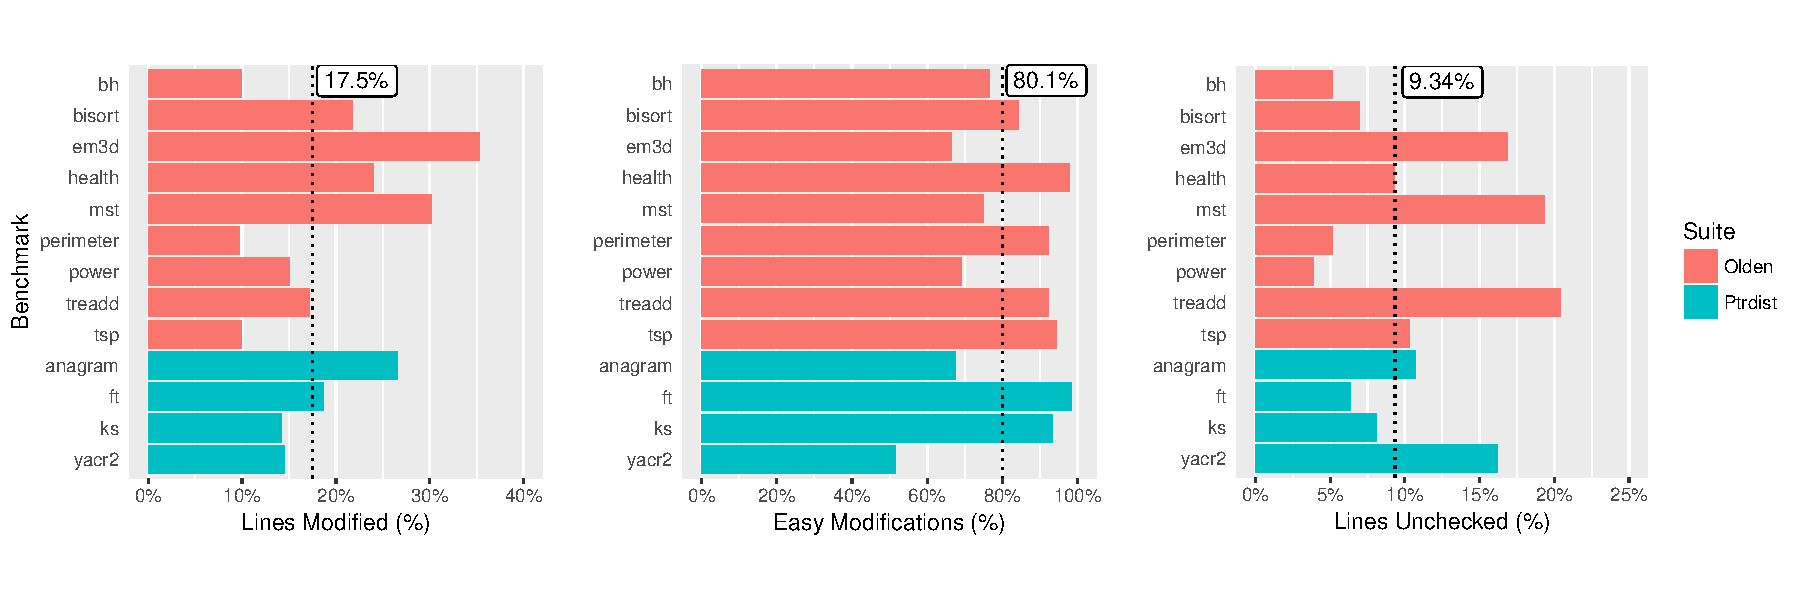
\includegraphics[width=\linewidth]{scripts/modifications}
\caption{Code Modifications}
\label{fig:cm-plot}
\end{figure}

On average, the changes modified \ResultLinesModifiedMean of benchmark
lines of code. Most of these changes were in declarations,
initializers, and type definitions rather than in the program logic.
In the evaluation of Deputy~\cite{Condit2007}, the reported figure of
lines changed ranges between 0.5\% and 11\% for the same benchmarks,
showing they have a lower annotation burden than Checked C.

We modified the benchmarks to use checked blocks and the top-level
checked pragma. We placed code that could not be checked because it
used unchecked pointers, or assignments where our static analysis
could not currently verify that the assignment was valid, in unchecked
blocks. On average, about \ResultLinesUncheckedMean of the code
remained unchecked after conversion, with a minimum and maximum of
\ResultLinesUncheckedMin and \ResultLinesUncheckedMax. The causes were
almost entirely variable argument functions such as
\lstinline|printf|.

We manually inspected changes and divided them into \emph{easy}
changes and \emph{hard} changes. Easy changes include:

\begin{itemize}
\item replacing included headers with their checked versions;
\item converting a \uncheckedptrT{} to a \PtrT{};
\item adding the \kwchecked{} keyword to an array declaration;
\item introducing a \kwchecked{} or \kwunchecked{} region;
\item adding an initializer; and
\item replacing a call to \lstinline|malloc| with a call to
\lstinline|calloc|.
\end{itemize}

Hard changes are all other changes, including changing a
\uncheckedptrT{} to a \ArrayptrT{} and adding a bounds declaration,
adding structs, struct members, and local variables to represent
run-time bounds information, and code modernization.

We distinguish between the two because we believe easy changes can be
automated (as with our automated \PtrT{} conversion tool) or made
unnecessary in the future by relaxing requirements such as the
additions of initializers.

In all of our benchmarks, we found the majority of changes were easy.
In six of the benchmarks, the only hard changes were adding bounds
annotations relating to the parameters of \lstinline|main|. In yacr2
there are a lot of bounds declarations that are all exactly the same
where global variables are passed as arguments, inflating the number
of ``hard'' changes.

\paragraph{Layout Changes} In three benchmarks---em3d, mst, and
yacr2---we had to add intermediate structs so that we could represent
the bounds on \ArrayptrT{}s nested inside arrays. In mst we also had
to add a member to a struct to represent the bounds on an
\ArrayptrT{}. In the first case, this is because we cannot represent
the bounds on nested \ArrayptrT{}s, in the second case this is because
we only allow bounds on members to reference other members in the same
struct. In em3d and anagram we also added local temporary variables to
represent bounds information.

\section{Performance Results}

\begin{figure}[ht]
\centering
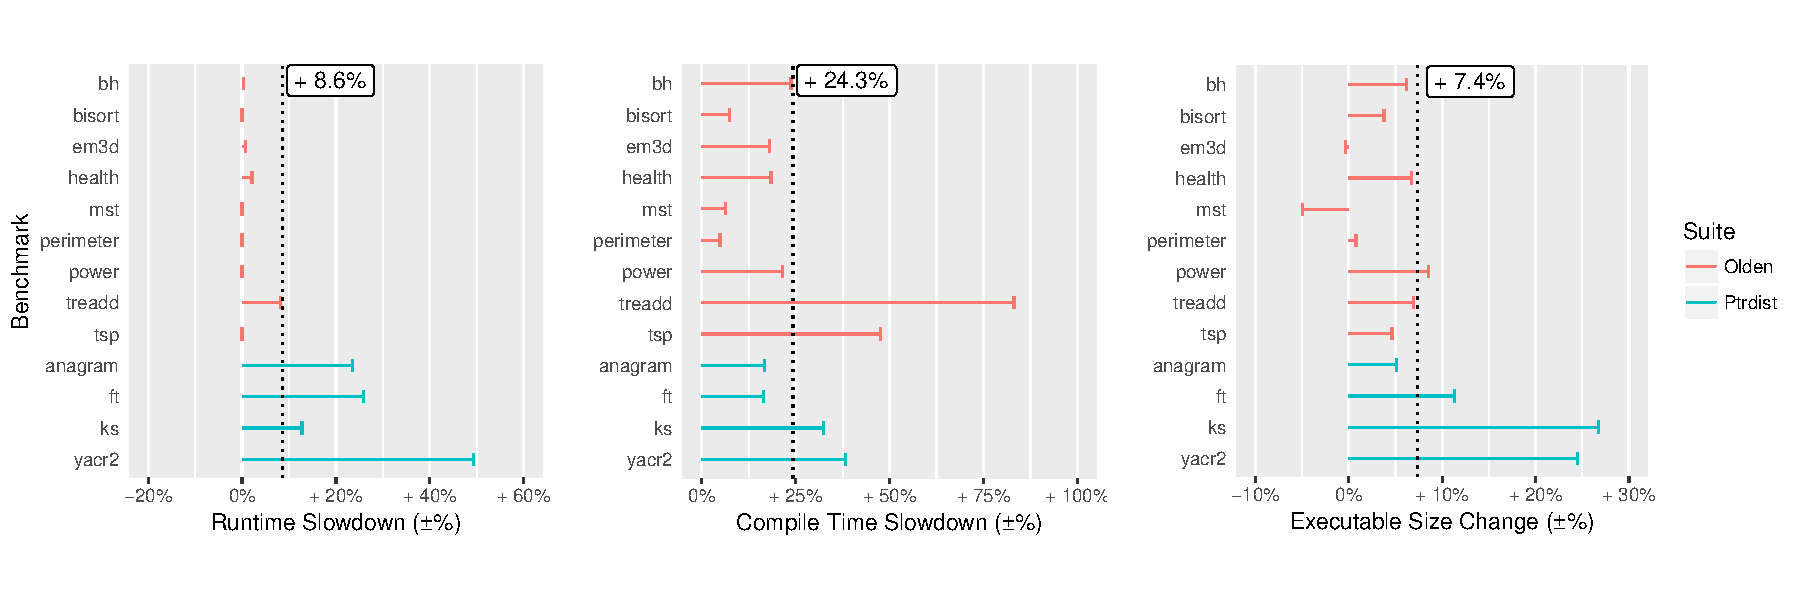
\includegraphics[width=\linewidth]{scripts/overheads}
\caption{Performance Overheads}
\label{fig:oh-plot}
\end{figure}

An important concern about run-time checking for C is the effect on
performance and compile time. The average run-time overhead introduced
by added dynamic checks was \ResultRunTimeMean. In more than half of
the benchmarks the overhead was less than 1\%. We believe this to be
an acceptably low overhead that better static analysis may reduce even
further.

In all but two benchmarks---treadd and ft---the added overhead matches
(meaning performance is within 2\% of) or betters that of Deputy. For
yacr2 and em3d, Checked C does substantially better than Deputy, whose
overheads are 98\% and 56\%, respectively. Checked C's overhead
betters or matches that reported by CCured in every case but ft.

On average, the compile-time overhead added by using Checked C is
\ResultCompileTimeMean. The maximum overhead is \ResultCompileTimeMax,
and the minimum is \ResultCompileTimeMin faster than compiling with C.
We have spent no time at all optimising compile-time for Checked C. In
particular, treeadd is a major outlier because the program is so
short.

We also evaluated code size overhead, by looking at the change in the
size of \lstinline|.text| section of the executable. This excludes data
that might be stripped, like debugging information. Across the
benchmarks, there is an average \ResultExecutableSizeMean code size
overhead from the introduction of dynamic checks. Ten of the programs
have a code size increase of less than 10\%.

\section{Evaluation}

All considered, we offer equivalent or better performance than either
CCured or Deputy provide, at the outlay of having to convert a larger
amount of code. We believe this to be a good trade-off, partially
because we feel most of these changes can be automated, and partially
because we provide the programmer greater control over how they
express their bounds in terms of other program data. The latter in
particular allows the programmer to work with their optimizer to
ensure run-time overhead, especially in tight loops, remains low.

\subsection{Interaction with the LLVM Optimizer}

Currently we have done no specific work within our compiler to elide
or optimize our dynamic checks. Any checks that Clang/LLVM currently
removes, it does so using its existing optimization passes.

We expected the LLVM optimizer to be a lot worse at optimizing dynamic
checks than it turned out to be. In only two of our benchmarks did we
have to hand-optimize these programs to reduce the overhead of dynamic
checking to approximately 0\%. This was accomplished by a mixture of
being more specific with annotated bounds (including introducing
temporary variables) and hoisting checks from inner loops using
explicit dynamic checks.

Expressions that caused most difficulty for removing dynamic checks
was code involving (at least) two pointer dereferences, as this incurs
an unavoidable non-null check on the inner pointer, even if the outer
pointer can be proven to be non-null. This can cause overhead in loops
iterating through, for example, linked lists or graphs. We are working
on a proposal to add nullness (and non-null) annotations to pointers
in Checked C, which would allow for these inner non-null checks to be
elided in many cases.

%%% Local Variables:
%%% mode: latex
%%% TeX-master: "tr02"
%%% End:

\chapter{Related Work}
\label{sec:related-work}

Attempting to make C memory safe is a well-trodden
path~\cite{Szekeres:2013:SEW:2497621.2498101}. Approaches fall into
four categories: better type systems; runtime representations of
bounds; static analysis annotations; and instrumentation. We avoid
mentioning approaches that propose new languages or operating-system
integration of protections.

\paragraph{Better Type Systems} In this approach, the compiler adds
new pointer types, perhaps including bounds information, with rules
that are enforced at compile time either by the type-checker or by
other static analyses. Any found errors prevent compilation from being
successful.

The largest influence on Checked C's approach is
Deputy~\cite{Condit2007}, a dependent-type system for C. This project
used dependent types for two reasons, the first is to represent array
bounds, the second is to ensure access to unions is via the correct
member. Unfortunately, to use Deputy, the programmer had to rewrite
their C program all at once, which is uneconomical and raises the
effort required to get any safety payoff. With our unchecked blocks
and interoperation types, we do not require the whole program to be
translated at once. The programmer also has little to no control over
the bounds expressions, preventing dynamic check optimizations.

CCured~\cite{Necula2005} takes a similar approach to ours, with new
pointer types to represent various kinds of arrays. They couple this
with an analysis of pointer usage which we have emulated in the
conversion tool described in~\cite{ruef2017draft}.

\paragraph{Run-time Representations of Bounds} In this approach, the
compiler uses extra memory to represent run-time bounds. This then
allows the compiler to insert checks which ensure pointers are within
bounds. They may also have to generate code to update bounds
information as other data within the program changes.

For instance, the SoftBound~\cite{Nagarakatte2009} work has a shadow
memory space where they store information about pointer bounds. In
order to achieve low run-time overhead, this approach requires up to
twice the memory of the original program, something that is not always
available on all platforms. Other work in the same
vein~\cite{Nagarakatte2015} uses hardware-based approaches that
require Memory Management Unit support.

CCured~\cite{Necula2005} also uses run-time representations for its
pointers, changing the in-memory layout, which we wanted to avoid. In
particular, pointer values are now represented by up to three
pointers, one for the pointer itself, and one each for its upper and
lower bounds. CCured also uses a garbage collector to implement sound
management of pointers it cannot infer information about, something we
have avoided the runtime overhead of.

\paragraph{Static Analysis Annotations} In this approach, the
programmer adds manual annotations to pointer declarations, similar to
our bounds expressions. These are then checked by an external static
analyser. The main difference is correct usage of these is enforced by
separate static analysis, and is not built into the original compiler.

The main solution in this space is SAL~\cite{MicrosoftSAL}, which can
detect, but not prevent bugs. Its annotations not only denote bounds,
but also whether a pointer may be read from or written to. SAL
includes annotations for function behaviour, such as locking, which we
do not include.

\paragraph{Instrumentation} Lastly, we have some dynamic analysis
systems that are not intended for production usage, but can detect
incorrect usage of the C language. They are intended for usage in
testing setups in conjunction with fuzzing systems that ensure the
dynamic analysis can reach most program points.

The two most prominent of these are ASan~\cite{Serebryany2012} and
UBSan~\cite{UBSan}. These can detect and prevent addressing and
undefined behaviour issues in C dynamically, including out-of-bounds
accesses and invalid pointer arithmetic.



%%% Local Variables:
%%% mode: latex
%%% TeX-master: "tr02"
%%% End:

\chapter{Conclusion}
\label{sec:conclusion}

This report has described how I implemented the dynamic checks in the
Checked C compiler. I have presented a flow-insensitive algorithm for
propagating bounds information through expressions, such that these
bounds can be checked when memory is accessed, and has shown one
possible compilation of these bounds expressions into dynamic checks.

I have also shown that, for a set of pointer-intensive benchmarks,
though the programmer will have to modify on average
\ResultLinesModifiedMean of each benchmark in order to have the
soundness Checked C guarantees, this gives a run-time overhead of on
average \ResultRunTimeMean and at most \ResultRunTimeMax.

This work is an important step towards proving the viability and
usefulness of Checked C.


%\section{Future Work}

%%% Local Variables:
%%% mode: latex
%%% TeX-master: "tr02"
%%% End:


\appendix
\addtocontents{toc}{%
  \protect\bigbreak
  {\large\bfseries \hfill Appendices\hfill }
  \protect\smallbreak
 }

\bibliography{checkedc}
\theendnotes
\chapter{C Syntax}
\label{app:c-syntax}

This appendix contains a definition of the relevant parts of C Syntax
for this report. This is based on the C11 Specification, but written
with mathematical symbols rather than ASCII text.

\begin{align*}
  \text{LValue Expressions} \\*
  e_l \gis {} & x  \tag*{Variables} \\
  \gor {} & \deref e_v \tag*{Dereference} \\
  \gor {} & e_v[e_v] \tag*{Index} \\
  \gor {} & e_l \member m \tag*{Struct Member Access} \\
  \gor {} & e_v \arrow m \tag*{Pointer Member Access} \\[1em]
%
\text{Value Expressions} \\*
  e_v \gis {} & \addrof e_l \tag*{Address-of} \\
  \gor {} & e_l \assign e_v \tag*{Assignment} \\
  \gor {} & e_l \compassign e_v \tag*{Compound Assignment} \\
  \gor {} & e_l \inc \mathrel{\mid} \inc e_l \tag*{Increment} \\
  \gor {} & e_l \dec \mathrel{\mid} \dec e_l \tag*{Decrement} \\
  \gor {} & e_v \member m \tag*{Struct Member Access} \\
  \gor {} & e_v , e_v \tag*{Comma Expression} \\
  \gor {} & e_v \binop e_v \tag*{Binary Operation} \\
  \gor {} & e_v \mathrel{R} e_v \tag*{Binary Relational Operation} \\
  \gor {} & \unop e_v \tag*{Unary Operation} \\
  \gor {} & e_v(\overline{e_v}) \tag*{Function Call} \\
  \gor {} & (t)e_v \tag*{Cast} \\
  \gor {} & e_v \mathrel{?} e_v : e_v \tag*{Conditional Operator} \\
  \gor {} & l \tag*{Literal Value} \\
  \gor {} & e_l \tag*{Lvalue \& Array Conversion} \displaybreak\\[1em]
  % 
  \text{Binary Operators} \\*
  \binop \gis {} & + \tag*{Addition} \\
  \gor {} & - \tag*{Subtraction} \\
  \gor {} & * \tag*{Multiplication} \\
  \gor {} & / \tag*{Division} \\
  \gor {} & \% \tag*{Modulus} \\
  \gor {} & \& \tag*{Bitwise AND} \\
  \gor {} & \mid \tag*{Bitwise OR} \\
  \gor {} & \wedge \tag*{Bitwise XOR} \\
  \gor {} & \gg \tag*{Bitwise Shift Right} \\
  \gor {} & \ll \tag*{Bitwise Shift Left} \\[1em]  
  % 
  \text{Relational Operators} \\*
  R \gis {} & \&\& \tag*{Logical AND} \\
  \gor {} & \mid\mid \tag*{Logical OR} \\
  \gor {} & \mathord{==} \tag*{Equality} \\
  \gor {} & \mathord{!=} \tag*{Negated Equality} \\
  \gor {} & \mathord{>} \mathrel{\mid}
             \mathord{\ge} \mathrel{\mid}
             \mathord{<} \mathrel{\mid}
             \mathord{\le} \tag*{Comparison} \\[1em]
  % 
  \text{Unary Operators} \\*
  \unop \gis {} & + \tag*{Unary Plus} \\
  \gor {} & - \tag*{Numerical Negation} \\
  \gor {} & \sim \tag*{Bitwise Negation} \\
  \gor {} & ! \tag*{Logical Negation} \\[1em]
  %
  \text{Literals} \\*
  l \gis {} & \mathtt{NULL} \tag*{Null Pointer Literal} \\
  \gor {} & \mathrm{integers} \tag*{Integer Literals} \\
  \gor {} & \mathrm{floats} \tag*{Float Literals} \\
  \gor {} & \{ l , \dots \} \tag*{Array \& Struct Literals} \\[1em]
  %
  \text{Types} \\*
  t \gis {} & \dots \\[1em]
  %
  \text{Struct Members} \\*
  m \gis {} & \dots \\
\end{align*}

%%% Local Variables:
%%% mode: latex
%%% TeX-master: "tr02"
%%% End:

\chapter{Propagation Rules}
\label{app:propagation-rules}

These are the algebraic definitions of our propagation algorithm to go
with the descriptions in~\autoref{sec:propagation-rules}. Certain
helper functions are explained in the text, rather than
algebraically.

\begin{figure}[ht]
\begin{align*}
  % Lvalue Bounds
  \lbounds(e_l) &\in \mbounds(e_v, e_v) \tag*{Lvalue Bounds} \\[1ex]
  \lbounds(x) &= \abounds(x, \mv{N}) \tag*{Variables} \\
                & \qquad \text{when } \typeof(x) = \arr(\mv{T}, \mv{N}) \\
                &= \sbounds(\addrof x) \text{ otherwise.} \\[1ex]
  \lbounds(\deref e_v) &= \vbounds(e_v) \tag*{Dereference} \\[1ex]
  \lbounds(e_1[e_2]) &= \vbounds(e_{base}) \tag*{Index} \\
                & \qquad \text{where } e_{base} = base(e_1, e_2) \\[1ex]
  \lbounds(e_l \member m) &= \abounds(e_l \member m, \mv{N}) \tag*{Struct Member Access} \\
                &\qquad \text{when } \typeof(e_l \member m) = \arr(\mv{T}, \mv{N}) \\
                &= \sbounds(\addrof (e_l \member m)) \text{ otherwise.} \\[1ex]
  \lbounds(e_v \arrow m) &= \abounds(e_v \arrow m, \mv{N}) \tag*{Pointer Member Access} \\
                &\qquad \text{when } \typeof(e_v \arrow m) = \arr(\mv{T}, \mv{N}) \\
                &= \sbounds(\addrof (e_v \arrow m)) \text{ otherwise.} \\[1em]
                %% Bounds Helpers/Sugar
  \sbounds(e_v) &= \mbounds(e_v, e_v + 1) \tag*{Single Object Bounds} \\
  \abounds(e_l, N) &= \mbounds(e_l, e_l + N) \tag*{Constant-sized Array Bounds} \\
                & \qquad \text{when } N \text{ is constant.} \\
  &= \mbounds(\text{unknown}) \text{ otherwise.}
\end{align*}
\caption[Lvalue Bounds Propagation]{Lvalue Bounds Propagation Rules (Mutually
Recursive with~\autoref{fig:val-bounds-prop})}
\label{fig:lval-bounds-prop}
\end{figure}


\begin{figure}[ht]
\begin{align*}
 % Value Bounds
  \vbounds(e_v) &\in \mbounds(e_v, e_v) \tag*{Value Bounds} \\[1ex]
  \vbounds(\mathtt{NULL}) &= \mbounds(\text{any}) \tag*{Null Pointer Literal} \\[1ex]
  \vbounds(l) &= \mbounds(\text{unknown}) \tag*{Other Literals} \\[1ex]
  \vbounds(\addrof e_l) &= \lbounds(e_l) \tag*{Address-of} \\[1ex]
  \vbounds(e_l \assign e_v) &= \vbounds(e_v) \tag*{Assignment} \\[1ex]
  \vbounds(e_l \compassign e_v) &= \ltbounds(e_l) \tag*{Compound Assignment} \\[1ex]
  \vbounds(e_l \inc) &= \ltbounds(e_l) \tag*{Increment \& Decrement} \\
                &\qquad \text{Likewise for all Increment \& Decrement operators} \\[1ex]
  \vbounds(e_v\member m) &= \srbounds(e_v, m) \tag*{Struct Member Operator} \\[1ex]
  \vbounds(e_f(\overline{e_{arg}})) &= \rbounds(e_f) \left[ \textrm{params}(f) \middle/ \overline{e_{arg}}\right] \tag*{Function Call}\\[1ex]
  \vbounds(e_{v1} , e_{v2}) &= \vbounds(e_{v2}) \tag*{Comma Expression} \\[1ex]
  \vbounds(e_l) &= \lbounds(e_l) \tag*{Array Conversion} \\
                &\qquad \text{when } \typeof(e_l) = \arr(\mv{T}, \mv{N}) \\
                &= \ltbounds(e_l) \text{ otherwise}
                  \tag*{Lvalue Conversion} \\[1ex]
  \vbounds(e_1 \binop e_2) &= \vbounds(e_{base}) \tag*{Pointer Arithmetic} \\
                &\qquad \text{when } e_1 \binop e_2 \text{ has pointer type} \\
                &\qquad \text{where } e_{base} = base(e_1, e_2) \\[1ex]
  \vbounds(e_1 \mathrel{R} e_2) &= \mbounds(\text{unknown}) \tag*{Binary Relational Operators} \\[1ex]
  \vbounds(! e_v) &= \mbounds(\text{unknown}) \tag*{Logical Negation Operator} \\[1ex]
  \vbounds(e_v) &= \vbounds(e_{vi}) \tag*{Other Expressions} \\
                &\qquad
                  \text{where } e_{vi}
                  \text{ is the subexpression of } e_v
                  \text{ with known bounds} \\
                &\qquad
                  \text{If more than one subexpression of } e_v
                  \text{ has known bounds,}\\
                &\qquad\quad
                  \text{all calculated bounds must be equal.} \\[1ex]
                &= \mbounds(\text{unknown}) \text{ otherwise}\\[1em]
  \rbounds(f) &\in \mbounds(e_v, e_v) \tag*{Bounds on Function Return} \\[1em]
  \srbounds(e_v, m) &\in \mbounds(e_v', e_v') \tag*{Struct Relative Bounds}
\end{align*}
\caption[Value Bounds Propagation Rules]{Value Bounds Propagation Rules (Mutually
Recursive with~\autoref{fig:lval-bounds-prop}
and~\autoref{fig:lval-target-bounds-prop})}
\label{fig:val-bounds-prop}
\end{figure}

\begin{figure}[ht]
\begin{align*}
%% Lvalue Target Bounds
  \ltbounds(e_l) &\in \mbounds(e_v, e_v) \tag*{Lvalue Target Bounds} \\[1ex]
  \ltbounds(e_l) &= \sbounds(e_l) \tag*{Checked Singleton Pointer Bounds}\\
                 &\qquad \text{where } \typeof(e_l) = \PtrT \\[1ex]
  \ltbounds(x) &= \dbounds(x) \tag*{Variable Target Bounds}\\[1ex]
  \ltbounds(e_l \member m) &= \srbounds(e_l, m) \tag*{Struct Member Target Bounds}\\
  \ltbounds(e_v \arrow m) &= \srbounds(e_v, m) \tag*{Pointer Member Target Bounds}\\[1ex]
  \ltbounds(\_) &= \mbounds(\text{unknown}) \\[1em]
  \dbounds(x) &\in \mbounds(e_v, e_v) \tag*{Declared Bounds}
\end{align*}
\caption[Lvalue Target Bounds Propagation Rules]{Lvalue Target Bounds
Propagation Rules}
\label{fig:lval-target-bounds-prop}
\end{figure}

%%% Local Variables:
%%% mode: latex
%%% TeX-master: "tr02"
%%% End:



\end{document}
